\chapter{Diskussion der Umsetzung}
\label{chap:five}
Im folgendem Kapitel wird das Design des Prototypen besprochen. Dabei wird zunächst auf die technischen Details der
Implementierung eingegangen. Danach folgt die Vorstellung der Systemarchitektur und der zugehörigen Teilsysteme.
Es wird aufgezeigt, wie die einzelnen Teilsysteme funktionieren und ineinandergreifen. Ausgewählte Programmcode-Beispiele sollen zum  
vertieften Verständnis beitragen.\footnote{\url{http://pfad/zu/github/repo}}

Im Anschluss daran wird die praktische Funktionsweise des Systems skizziert. Neben den technischen Voraussetzungen wird dabei 
die Vorgehensweise des Datenimports beschrieben sowie auf das Layout und die Darstellung der Daten im Dashboard eingegangen. 
Abschließend findet anhand der Anforderungen und der Anwendungsfälle, die im \autoref{chap:four} formuliert sind, eine Bewertung des Systems statt.
%Dabei wird auf die allgemeine Bewertung und auf die Datengrundlage kurz eingegangen.


\section{Implementierung}
    
    \subsection{Technische Details der Implementierung}
    Das Proof-of-Concept wurde mittels der Programmiersprache Python umgesetzt.
    Python ist eine höhere Programmiersprache. Sie ist weitverbreitet \cite[vgl.][]{loukides_where_2021} und besitzt
    eine einfache Syntax. Besonderheiten von Python sind der Verzicht auf geschweifte Klammern und Interpunktionen nach Anweisungen.
    Die Anweisungen sind durch Einrückungen strukturiert und nicht durch öffnende und schließende Klammern
    getrennt. Des Weiteren zeichnet sich Python durch eine dynamische Typisierung aus und ist dadurch sowohl für Skripte als auch 
    für die schnelle Entwicklung von Anwendungen geeignet. Python erlaubt die Aufteilung von Programmen in Modulen, die in anderen Python-Programmen wiederverwendet werden können
    \cite[vgl.][]{python_6_2021}.
    % Sie ist für alle wichtigen Plattformen frei verfügbar und verfügt über eine große Dokumentation \cite[vgl.][]{python_welcome_2021}.
    Wie andere Programmiersprachen besitzt Python eine umfangreiche Standardbibliothek.
    Daneben gibt es noch eine Vielzahl von Modulen, Programmen und Werkzeugen von Drittanbietern \cite[vgl.][]{python_pypi_2021}.
    Mit den \acrfull{PEP8} steht außerdem noch ein übersichtlicher Style Guide für den Python-Code bereit, indem die Formatierungsrichtlinien für die bessere Lesbarkeit und Konsistenz des Programmcodes formuliert sind \cite[vgl.][]{rossum_pep_2021}.

    %Genutzt wurde für das Projekt insbesondere die Python-Bibliothek pandas, die eine Open-Source-Bibliothek für Datenanalyse und 
    %Datenmanipulation darstellt \cite[vgl.][]{pandas_pandas_2021}. 
    Wichtige Konzepte dieser Bibliothek sind der pandas Dataframe\footnote{Die Bezeichnung für einen Dataframe im Programmcode ist nach pandas-Konventionen \texttt{df}.} und die pandas Series, die pandas Objekte sind. Der pandas Dataframe ist eine zweidimensionale 
    tabellarische Datenstruktur mit beschrifteten Achsen (Spalten und Zeilen). In ihn
    werden die Daten unter anderem aus csv- oder xlsx-Dateien über pandas Funktionen geladen.
    Eine pandas Series kann Bestandteil eines Dataframes sein. Der Datentyp entspricht dem eines eindimensionalen Arrays. 
    \autoref{fig:pandas Dataframe und pandas Series} zeigt anhand der Umsatzdaten die ersten fünf Reihen
    eines pandas Dataframe und einer pandas Series desselben Dataframes. 
    
    
    \begin{figure}[H]
        \centering
            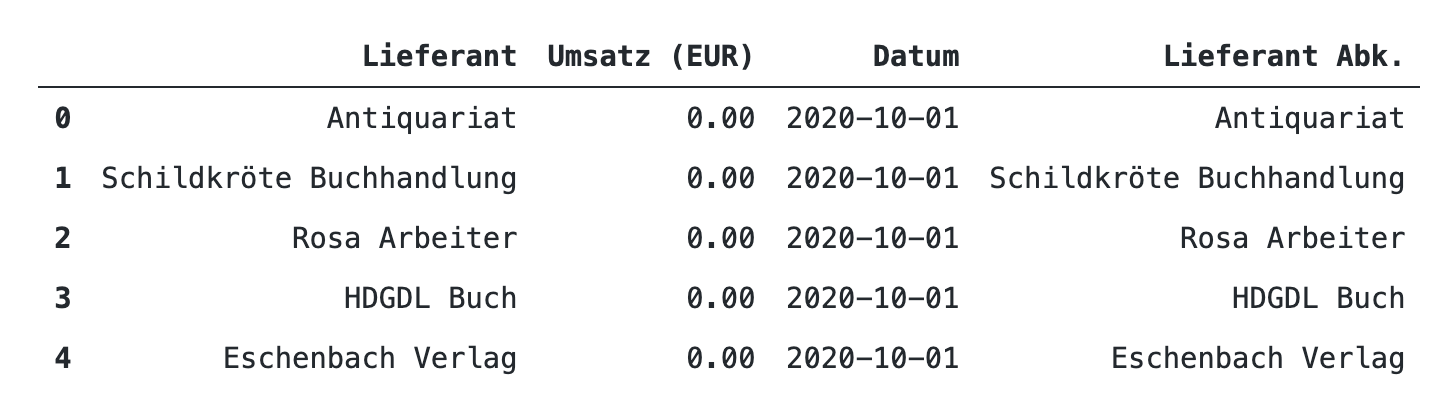
\includegraphics[width=7.5cm, height=4.0cm]{dataframe_example}
            \hspace{1cm}
            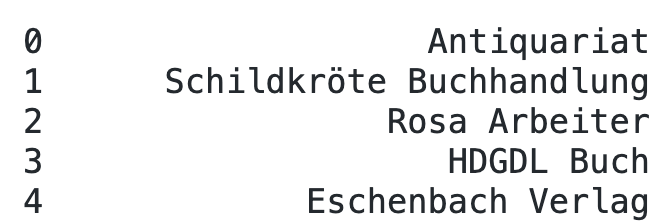
\includegraphics[width=5.0cm, height=4.0cm]{series_example}
            \caption{pandas Dataframe (links) und pandas Series (rechts)}
            \label{fig:pandas Dataframe und pandas Series}
    \end{figure}

    Der Zugriff auf die Series kann über den Spaltenkopf \enquote{Lieferant Abk.} oder indexbasiert erfolgen. 
    Sowohl der Dataframe als auch die Series haben einen Index, über den auf die einzelnen Werte zugegriffen werden kann. 
    
    Auf dem Dataframe, der als sogenannter Container für die Series dient, können verschiedene Operationen der Datenanalyse und 
    -manipulation erfolgen. Ähnlich wie bei Abfragen einer Datenbank lassen sich verschiedene Funktionen wie \texttt{sort()}- oder \texttt{groupby()}
    in Zusammenhang mit Aggregatfunktionen wie \texttt{mean()}, \texttt{median()} oder \texttt{sum()} auf den Series durchführen.
    Auch gibt es eine Vielzahl von Funktionen, um Daten rasch zu explorieren. Zum Beispiel bietet sich Jupyter Notebook als
    Entwicklungsumgebung dazu hervorragend an, da in dieser der Code zeilenbasiert ausgeführt werden kann.\footnote{Für das vorliegende Projekt wurden 
    insbesondere Teile der Datenanalyse damit entwickelt und getestet.} Die Werte der Zellen können verschiedene Datentypen
    annehmen. Zum Beispiel können die Datumswerte der Spalte \enquote{Datum} in Datetime-Objects umgewandelt werden.

    In Verbindung mit pandas ist Python neben \textsf{R} im wissenschaftlichen Kontext für Data-Science-Projekte deshalb sehr beliebt.
    
    Es gibt eine Vielzahl an Bibliotheken für Python, die für die Entwicklung von interaktiven Datenvisualisierungen verfügbar sind. Zu
    nennen wären Bokeh \cite[vgl.][]{van_de_ven_bokeh_2021}, Altair \cite[vgl.][]{altair_altair_2021} und die 
    Graphic Libraries von Plotly \cite[vgl.][]{plotly_plotly_2021}.
    Plotly Express ist eine Graphische Bibliothek für Python, \textsf{R} und Javascript. Es ist eine Weiterentwicklung (Wrapper) der Bibliothek Plotly Graph Objects. 
    Plotly Express besitzt eine einfachere Syntax bei fast annäherender Feature-Gleichheit mit Plotly Graph Objects.\cite[][]{plotly_plotly_2021}.
    So können mit wenigen Zeilen Python-Code interaktive Grafiken erzeugt werden. 
    An interaktiven Basisfunktionalitäten bietet Plotly Express zum Beispiel Hover-Informationen der Datenpunkte, Zoom-In und Zoom-Out-Möglichkeiten,
    das Aus- und Abwählen von Balken oder Linien in den entsprechenden Diagrammen. Plotly Express kann pandas Dataframes 
    oder pandas Series als Datenobjekte erwarten und verarbeiten. Dabei können die Spaltenköpfe die Achsen darstellen 
    und die einzelnen Werte der Spalten die Datenpunkte bilden. Die Rendering-Engine für die Diagramme beruht auf dem JavaScript Framework D3.js. 
    Plotly Express ist frei verfügbar. In Kombination mit der Bibliothek Dash für die Entwicklung von interaktiven Dashboards lässt sich Plotly Express gut anwenden, 
    da beide von der selben Firma entwickelt werden und aufeinander abgestimmt sind.  Für das Projekt wurde sich deswegen für Plotly Express entschieden 
    und dieses hauptsächlich genutzt. 
    
    Mit der Bibliothek Dash wurde das Dashboard realisiert. Dash baut auf den Technologien Flask, plotly.js und React.js auf. Das Framework ermöglicht die Erstellung interaktiver Webapplikationen 
    oder \enquote{Analytical Applications} in Python ohne hierfür mit Javascript programmieren zu müssen \cite[vgl.][]{plotly_dash_2021}.
    Es gibt verschiedene Dash-Komponenten, die unterschiedliche Funktionen erfüllen. \texttt{dash\_html\_components} stellen Klassen für alle HTML-Elemente bereit.
    Die Schlüsselwortargumente dieser Klasse beschreiben HTML-Attribute wie style, className und id \cite[vgl.][]{plotly_dash_2021-2}. 
    Andere Komponenten sind \texttt{dash\_core\_components} oder \texttt{dash\_dependencies} \cite[vgl.][]{plotly_dash_2021-1}.
    \footnote{Die beiden Module \texttt{dash\_html\_components} und \texttt{dash\_core\_components} werden nach Python-Konventionen als \texttt{html} für die \texttt{dash\_html\_components} und als \texttt{dcc} für die \texttt{dash\_core\_components} bezeichnet und importiert.}
    Während die \texttt{dash\_core\_components}
    Steuerelemente und Graphen erzeugen, regeln die \texttt{dash\_dependencies} über Callback-Dekorator-Funktionen die Interaktion zwischen den einzelnen Komponenten.
    So kann zum Beispiel in der Dash-Webapplikation das Verhalten eines Diagramms von den Werten eines Dropdown-Menu gesteuert werden. 
    % Die zugehörige Callback-Dekorator-Funktion wird in diesem Falle automatisch von Dash aufgerufen, sobald sich der Wert des Dropdown-Menüs ändert. 
    %Dabei bewältigt Dash alle Javascript-Anforderungen im Front- und im Backend \cite[vgl.][]{plotly_dash_2021-3}.
    \texttt{dash\_bootstrap\_components} ist eine weitere Bibliothek, die zum Einsatz in diesem Projekt kommt. Sie unterstützt die grafische Umsetzung
    des Dashboardes \cite[vgl.][]{faculty_dash_2021}.

    \autoref{tab:Software-Requirements} zeigt einen kurzen Überblick über die Versionsnummern der genutzten Programmiersprache und der hauptsächlich 
    genutzten Bibliotheken sowie deren Open-Source Lizenzen.
    
    \begingroup
        \setlength{\tabcolsep}{4pt} % Default value: 6pt
        \renewcommand{\arraystretch}{1.0}
        %\resizebox{\textwidth}{!}{
        \begin{table}[H]
            \centering
            \begin{adjustbox}{max width=\textwidth}
            \Huge
            \begin{tabular}{lccl}
              %\begin{tabular}{p{3cm}p{5cm}p{1cm}p{1.5cm}p{2cm}p{4cm}}
               \toprule
               \textbf{Name}             &{Version}    &\textbf{Lizenz}                        & \textbf{Webseite}\\
               \midrule     
                    Python               &3.7.9         &Open Source (PSF)                     & \url{https://docs.python.org/3.7/}\\
                    pandas               &1.1.5         &3-Clause-BSD-License                  & \url{https://pandas.pydata.org/pandas-docs/version/1.1.5/}\\
                    Plotly               &4.14.1       &MIT-License                           & \url{https://plotly.com/python/}\\
                    Dash                 &1.18.1        &MIT-License                           & \url{https://dash.plotly.com/}\\


                \bottomrule
            \end{tabular}
            \end{adjustbox}
            \caption
            \label{tab:Software-Requirements}
            }
             \end{table}
        \endgroup
    

    \subsection{Systemarchitektur}
    
    Das System teilt sich in drei Teilsysteme auf, die im \autoref{chap:five_one_three} näher beschrieben und mit Beispielen erläutert werden. 
    %Teilsystem 4 besteht dahingegen wieder aus objekt-orientierter Programmierung. Genutzt wird hier eine Library, die OOP vorgibt. 
    In der folgenden \autoref{fig:Systemarchitektur} wird die Systemarchitektur des Projektes gezeigt.\footnote{Die schwarzen Pfeile zeigen vereinfacht
    den Datenfluss an.}

    \begin{figure}[H]
        \centering
            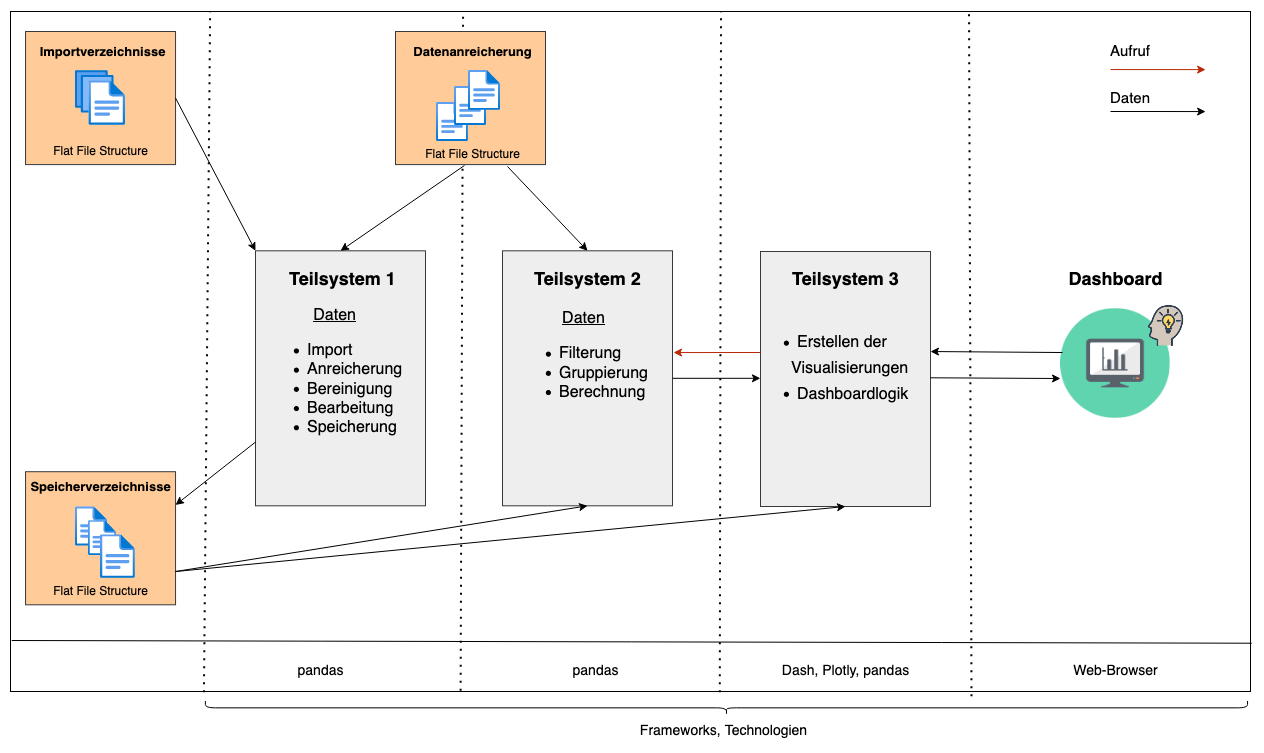
\includegraphics[width=14cm, height=12cm]{Systemarchitektur}
            \caption{Systemarchitektur}
            \label{fig:Systemarchitektur}
    \end{figure}

    Das Ziel des Teilsystems 1 ist es, die Daten aus heterogenen Datenquellen in einem einheitlichen Dateiformat zu speichern.
    Das Teilsystem 1 importiert die Daten zunächst aus den Datenquellen und unterwirft sie einem Transformationsprozess, der die Bearbeitung der Daten, die Berechnung
    auf den Daten und die Bereinigung der Daten umfasst. In Abhängigkeit von der Vielschichtigkeit der vorliegenden Daten bedarf dieser Prozess unterschiedlich vieler Transformationsschritte.  
    %Das Teilsystem 1 funktioniert zudem autonom vom Teilsystem 2 und Teilsystem 3. 
    Anschließend werden die in einem einheitlichen Format vorliegenden Daten durch das Teilsystem 2 
    für die Anzeige im Dashboard vorbereitet, indem das Teilsystem 2 mit der Python-Bibliothek pandas die Daten vorfiltert und Berechnungen auf den Daten ausführt. 
    Zudem wird auch noch eine Datenanreicherung vollzogen. Teilsystem 3 ist für das Layout des Dashboards, die Erstellung der Diagramme, die Anordnung der Diagramme im Dashboard und 
    die Bereitstellung von Interaktionen auf dem Dashboard verantwortlich. Die Daten aus dem Teilsystem 2 werden dem Teilsystem 3 übergeben,
    indem das Teilsystem 3 die Filterungen und Berechnungen des Teilsystems 2 aufruft. Teilsystem 3 sorgt für die Übergabe der Daten an das Dashboard zur dessen Anzeigezeit.
    
    Teilsystem 1 und Teilsystem 2 wurde objektorientiert programmiert, da hier der Anspruch bestand, den Programmcode
    für verschiedene Daten wiederzuverwenden. Teilsystem 3 besteht vorerst nur aus Funktionen, die die Anzeige im Frontend ermöglichen.
    \autoref{tab:Teilsysteme} zeigt die drei Teilsysteme mit einer Kurzbeschreibung der Hauptaufgabe.

       \begingroup
            \setlength{\tabcolsep}{4pt} % Default value: 6pt
            \renewcommand{\arraystretch}{1.5}
            %\resizebox{\textwidth}{!}{
            \begin{table}[h]
                \centering
                \begin{adjustbox}{max width=\textwidth}
                \Huge
                \begin{tabular}{cll}
                  %\begin{tabular}{p{3cm}p{5cm}p{1cm}p{1.5cm}p{2cm}p{4cm}}
                   \toprule
                   \textbf{Teilsystem}             & Name   &{Hauptaufgabe} \\
                   \midrule     
                            1                      &Import  &Import und erste Bereinigung der Daten aus heterogenen Datenquellen.\\
                            2                      &Datenbearbeitung     &Aufbereitung der Daten für die graphische Darstellung im Dashboard.\\
                            3                      &Darstellung          &Umwandlung der Daten in Datenvisualisierungen und Implementierung der Dashboard-Logik.\\
                        %   4                      &Standardbericht      &Export ausgewählter Datenvisualisierungen und Darstellung in Berichtsform.\\

                    \bottomrule
                \end{tabular}
                \end{adjustbox}
                \caption
                \label{tab:Teilsysteme}
                }
                 \end{table}
            \endgroup

    \subsection{Teilsysteme}
    \label{chap:five_one_three}
    
    \clearpage
    \textit{Teilsystem 1 Import}\\
    \begin{figure}[H]
        \centering
            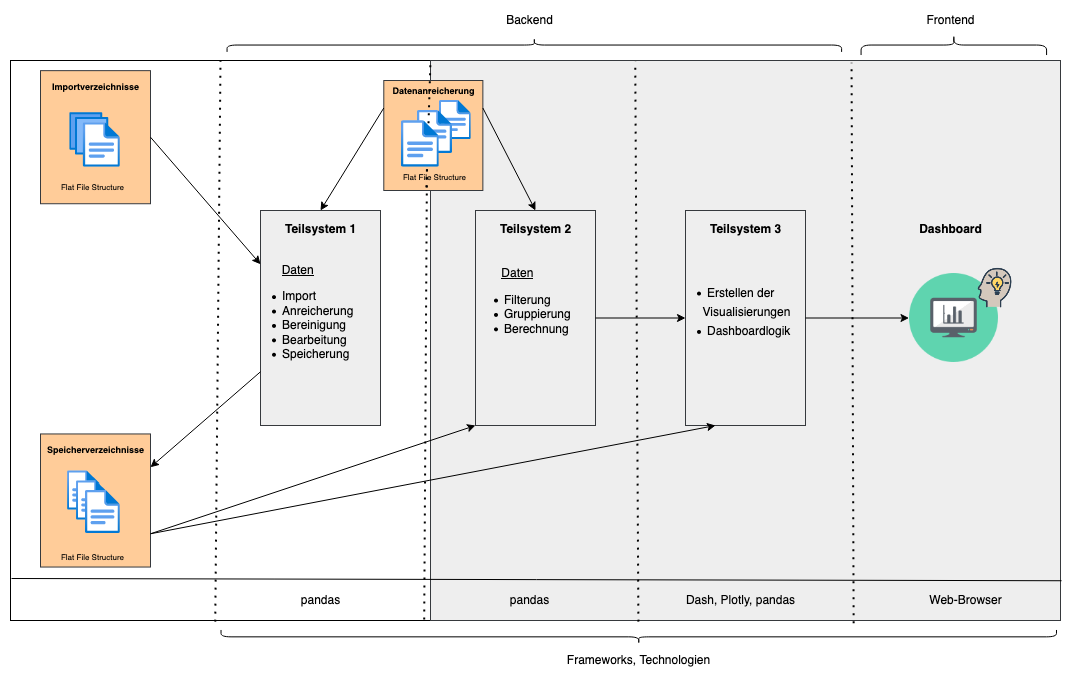
\includegraphics[width=15cm, height=10cm]{Systemarchitektur_Ts1}
            \caption{Systemarchitektur Teilsystem 1}
            \label{fig:Systemarchitektur Teilsystem 1}
    \end{figure}


    Das \textit{Teilsystem 1 Import} ist verantwortlich für den Import der Daten im Rohformat aus vordefinierten Importverzeichnissen 
    in vordefinierte Zielverzeichnisse. Das Layout der Importverzeichnisse ist eine Struktur, die für alle Daten, die importiert werden sollen,
    jeweils einen lokalen Ordner vorsieht. So zum Beisiel gibt es jeweils einzelne Ordner für bibliotheksspezifischen Daten wie zum Beispiel Budget- und Umsatzdaten.
    Da anhand der Dateinamen nicht unterschieden werden kann, um welche Daten es sich handelt, wurde diese Struktur eingeführt. 
    \footnote{Der Dateiname der semantisch einem Datumsformat entspricht, wird als Zusatzinformation mit den Daten abgespeichert, bei denen das Datum als Information benötigt wird.
    Anhand dieser Information werden im Teilsystem 2 mitunter die Daten gefiltert.} 
    Da es sich um Daten aus heterogenen Datenquellen handelt, unterscheiden sich die Daten durchaus in dem Dateiformat. 
    Das Teilsystem 1 unterstützt bereits den Import der Daten in Formaten wie txt, tsv, xlsx und xls. Diese Formate werden im Teilsystem 1 festgelegt
    und können noch um andere erweitert werden.
    
    Das Ziel des Teilsystems 1 ist einerseits die Daten automatisch ohne Informationsverlust zu importieren 
    und andererseits diese für die weitere Analyse mit notwendigen Daten wie zum Beispiel mit den Daten 
    der \textit{\acrshort{RVK}}-Fachsystematiken anzureichern.\footnote{Das Beispiel wird weiter unten noch ausführlich erläutert.}
    Ferner werden erste Bereinigungen der Daten wie zum Beispiel das Entfernen unnötiger Zeichen durchgeführt. Die Daten werden zum Abschluss im csv-Format abgespeichert. 
    Dabei werden die Daten ebenfalls in der Zeichenkodierung utf-8 gespeichert, um eine einfache syntaktische Homogenität zu gewährleisten. Das Layout der Speicherverzeichnisse
    entspricht dem Layout der Importverzeichnisse. Die Daten liegen in diesen Ordnern jeweils in einer Datei vor, die mit jedem Importprozess um die zu importierenden Daten wächst.

    Mit dem Teilsystem 1 soll eine einheitliche Datengrundlage für die spätere Bearbeitung und Darstellung der Daten garantiert werden. Für das csv-Format wurde sich aufgrund seiner flachen und einfachen Struktur, der guten Lesbarkeit
    und seiner weiten Verbreitung entschieden. Zu vergleichen wäre die Organisation der Speicherung mit einem Data Lake, nur dass hier die Daten in einem Dateiformat vorliegen.
    % Die Daten werden jeweils in ein pandas Dataframe geladen. Das Dataframe wird dann verschiedentlich bearbeitet, bevor es zum Schluss als csv-Datei in dem jeweiligen
    % Zielverzeichnis abgespeichert wird.
    
    Das \textit{Teilsystem 1 Import} besteht aus vier Klassen. Die \autoref{fig:classes import} zeigt die einzelnen Klassen mit ihren Methoden.
    Die Klassen im \textit{Teilsystem 1 Import} sind auf die Daten aus fremden Quellen zugeschnitten
    (Budget, Umsatz, Neuerwerbungslisten und Ausleihe (Anwendungsfall 2, 4-6)). Dennoch können mit mit ihnen auch die bibliotheksinternen Daten
    wie Lesesaalnutzung (Anwendungsfall 3) bearbeitet werden. 
    \begin{figure}[H]
        \centering
            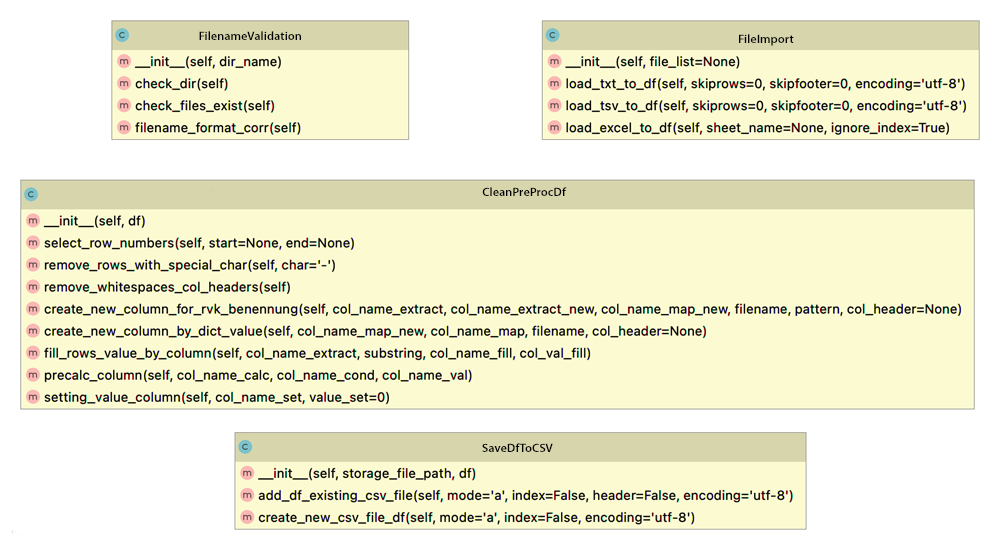
\includegraphics[width=15cm, height=12cm]{data_import_class1}
            \caption{Klassendiagramm - Teilsystem 1 Import}
            \label{fig:classes import}
    \end{figure}

    Instantiiert werden die einzelnen Klassen für die jeweiligen konkreten bibliothekarischen Daten in eigenen Python-Skripten. 
    So gibt es Skripte für Budget, Umsatz, Ausleihe und Bestand/Neuerwerbungen. Diese verwenden für die Daten passende Methoden
    und führen den Import durch.
    Den Ablauf des Teilsystems zeigt schematisch die \autoref{fig:flow import}.

    \begin{figure}[H]
        \centering
            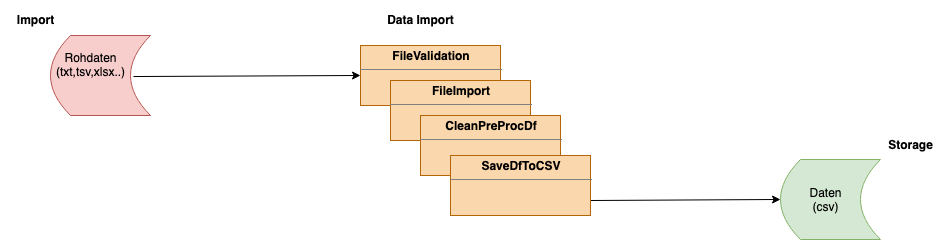
\includegraphics[width=13cm, height=8cm]{flow_imp}
            \caption{Datenfluss - Teilsystem 1 Import}
            \label{fig:flow import}
    \end{figure}

    
    (1) Für den ersten Schritt sind die Klassen \texttt{FilenameValidation} und \texttt{FileImport} verantwortlich.
    Die Dateien werden aus einem lokalen Verzeichnis in ein pandas Dataframe geladen. 
    Dabei wird mit den Methoden der Klasse \texttt{FilenameValidation} überprüft, ob sowohl das Verzeichnis als auch die Dateien existieren.
    Die Pfade für die zu überprüfenden Verzeichnisse werden vom Projektverzeichnis abgeleitet und in der \texttt{configuration.py} festgelegt.
    
    Des Weiteren wird sichergestellt, dass die Dateinamen einem definierten semantischen Format wie dem Datumsformat YYYY\_MM\_DD und 
    einem Dateiformat wie txt-, xlsx- oder tsv-Format entsprechen. Wenn die Daten nicht diesen Vorgaben entsprechen, werden sie nicht in
    das pandas Dataframe geladen. Da die Daten unterschiedlich aufgebaut und in unterschiedlichen Dateiformaten vorliegen, 
    werden beim Laden in den Dataframe jeweils verschiedene Methoden angewandt. Dabei werden spezifische pandas-Funktionen für 
    txt-Dateien oder für xlsx-Dateien eingesetzt, die diese Dateiformate parsen können. 
    Der Parser versucht die Datentypen der Werte in den Spalten aus den vorliegenden Werten der Spalten automatisch abzuleiten. 
    Dabei arbeitet er einen Datentyp nach dem anderen ab. Datentypen in pandas sind zum Beispiel int64, float64 oder objects. 
    Diese entsprechen ähnlichen Python-Typen wie int (int64), float (float64) oder auch Strings (objects). Daneben gibt es noch spezielle pandas Datentypen wie die bereits erwähnten Datetime-Objects, die aber nicht automatisch zugewiesen werden.
    Zunächst versucht pandas die Werte in Integerwerte zu konvertieren. Tritt in diesem Prozess ein Fehler auf, 
    wird zum nächsten Datentyp übergegangen. Wenn kein spezifischer Datentyp erkannt wird , werden die Werte in den Datentyp objects konvertiert \cite[Vgl.][]{golubin_how_2021}.
    \footnote{Die Erkennung des Datentyps funktioniert durchaus auch für andere Dateiformate und nur für csv-Formate. Das gelang für das vorliegende Projekt gut, sodass
    bei diesem Prozess nicht manuell eingegriffen wurde.}
    
    Beim Ladeprozess der Dateien in den pandas Dataframe wird mit den Methoden \texttt{load\_txt\_to\_df()} oder \texttt{load\_tsv\_to\_df()} 
    der Klasse \texttt{FileImport} der Dateiname von der Datei extrahiert und in einer neu geschaffenen Spalte des Dataframes im Datumsformat YYYY-DD-MM gespeichert.
    Anhand der Werte dieser Spalte werden später verschiedene Datenanalysen und Datenvisualisierungen vollzogen.\footnote{Dieses Verfahren wird bei den Daten ausgeführt, die einer zusätzlichen Datumsspalte bedürfen.} 
    Verantwortlich für die Extrahierung des Dateinamens ist die in \texttt{utils.py} ausgelagerte Funktion \texttt{date\_from\_filename()},
    die den Dateinamen als Argument entgegennimmt.\footnote{In der Datei \texttt{utils.py} sind noch andere Funktionen als stand-alone-functions für den Datenimport und Datenbearbeitung gruppiert,
    da diese das Objekt \texttt{self} nicht verändern. Zu finden ist die Datei im Projekt in dem Verzeichnis \texttt{src}.} 
    
    (2) Das geladene pandas Dataframe wird im zweiten Schritt durch die Klasse \texttt{CleanPreProcDf} aufgenommen und durch verschiedene Methoden dieser Klasse
    manipuliert. Beispielhaft ist hier die Methode \texttt{create\_new\_column\_for\_rvk\_benennung()} zu nennen, die aus einer Spalte einen Substring unter
    zuhilfenahme eines regulären Ausdruckes extrahiert, diesen in eine neue Spalte schreibt und ihn um zusätzliche Informationen anreichert. 
    Diese Methode wird sowohl bei den Neuerwerbungs/Bestandsdaten als auch bei den Ausleihdaten zweimal angewendet, um die  \textit{\acrshort{RVK}}-Fachsystematiken der
    Titelsignaturen zu extrahieren und durch die \textit{\acrshort{RVK}}-Benennungen anzureichern. 
    Zunächst werden die Untergruppen der Fachsystematiken aus der Signatur extrahiert, in einer neuen Spalte gespeichert und um die entsprechenden Benennungen der Untergruppen der 
    \textit{\acrshort{RVK}} angereichert. 
    Danach werden die Fachsystematiken aus den Untergruppen extrahiert und ebenfalls um die entsprechenden Bennungen angereichert.
    Mit der \autoref{fig:extr Fachsystematik} lässt sich dieser Prozess an der Signatur \enquote{CP 2000 zit 2018} nachvollziehen.
    \begin{figure}[H]
        \centering
            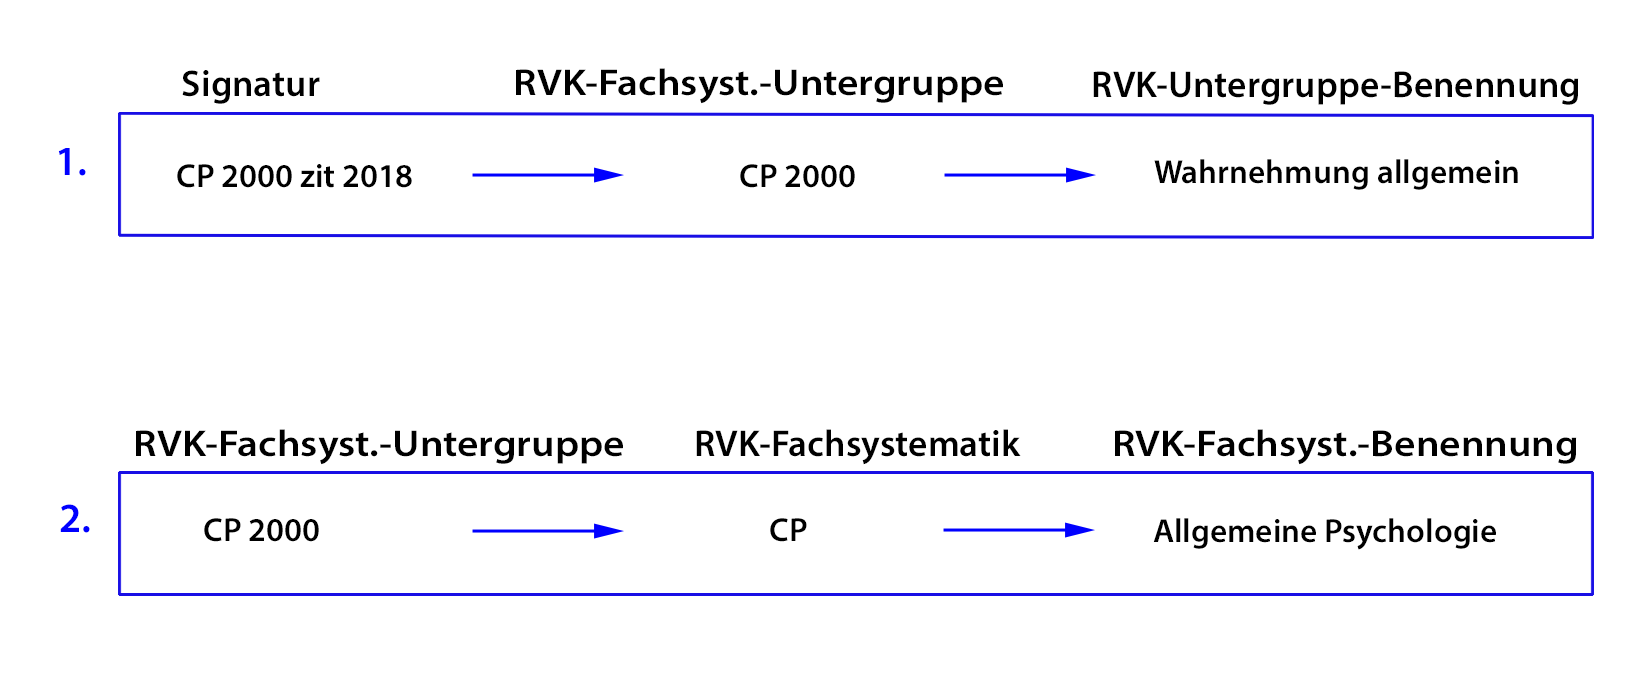
\includegraphics[width=14cm, height=6cm]{signatur_extr}
            \caption{Beispiel Extraktion Fachsystematik}
            \label{fig:extr Fachsystematik}
    \end{figure}

    Zu diesem Zweck liegt eine csv-Datei der \textit{\acrshort{RVK}} zu Grunde, die mit einem Python-Skript\footnote{Das Skript liegt im Projektverzeichnis
    unter \texttt{data/helper\_files}} aus einer \textit{\acrshort{RVK}}-XML-Datei entstanden ist.
    Diese XML-Datei kann von der \textit{\acrshort{RVK}}-Homepage bezogen werden und wird ungefähr vierteljährlich aktualisiert \cite[Vgl.][]{rvk_rvk_2021}.
    In dieser liegen die Fachsystematiken und die Untergruppen mit ihren Benennungen vor.\footnote{Manuell ergänzt wurde diese noch um selbstgeschaffene Fachsystematiken der Institutsbibliothek.}
    Diese wird bei jedem Aufruf der Methode mit den Werten der neu entstanden Spalte gemappt. Die Benennungen werden ebenfalls in je einer Spalte gespeichert.
    Ziel ist es, die Neuerwerbung- und Bestandsdaten später nach den \textit{\acrshort{RVK}}-Fachsystematiken und deren Untergruppen auszuwerten.
    
    
    Bei Umsatz- und Budgetdaten entstehen ebenfalls neue Spalten. In Bezug auf die Darstellung der Daten im Dashboard werden
    hier die Namen der Lieferanten und Kostenstellen in lesbarer Form in einer neuen Spalte gespeichert. 
    Des Weiteren gibt es in der Klasse \texttt{CleanPreProcDf} Methoden, die für die Entfernung von Zeilen mit bestimmten syntaktischen Zeichen wie Bindestrichen 
    verantwortlich sind oder die eine Vielzahl unnötiger Leerzeichen in Spaltenköpfen löschen  und durch ein Leerzeichen ersetzt.
    Ferner wird eine Berechnung durch die Methode \texttt{precalc\_column()} auf den Ausleihdaten ausgeführt.
    \footnote{Im Arbeitsprozess der Medienerschließung validiert die Bibliothek die RFID-Etiketten der Medien durch einmalige Ausleihe der Medien am Selbstverbucher.
    Deswegen wird die Anzahl der Ausleihe pro Medium um eins reduziert, wenn sie ein oder mehrmals ausgeliehen wurden.}
     
    (3) Nach dem Transformationsprozess wird das veränderte pandas Dataframe als csv-Datei in einem vorher definierten Speicherordner gespeichert. 
    Verantwortlich ist dabei die Klasse \texttt{SaveDFToCSV} mit den zwei Methoden \texttt{add\_df\_existing\_csv\_file()} und 
    \texttt{create\_new\_csv\_file\_df()}. 
    Es wird durch diese Methoden entweder eine neue csv-Datei mit dem Dataframe erstellt oder der Dataframe wird an eine bereits vorhandene csv-Datei angehängt.
    \autoref{fig:umsatzuebersicht_txt} zeigt die Original-Umsatz-Datei, die im txt-Format gespeichert wurde. Die anschließende Transformation durch das Teilsystem 1
    verwandelt die Datei in eine csv-Datei, die in \autoref{fig:umsatzuebersicht_csv} zu sehen ist.

    \begin{figure}[H]
        \centering
            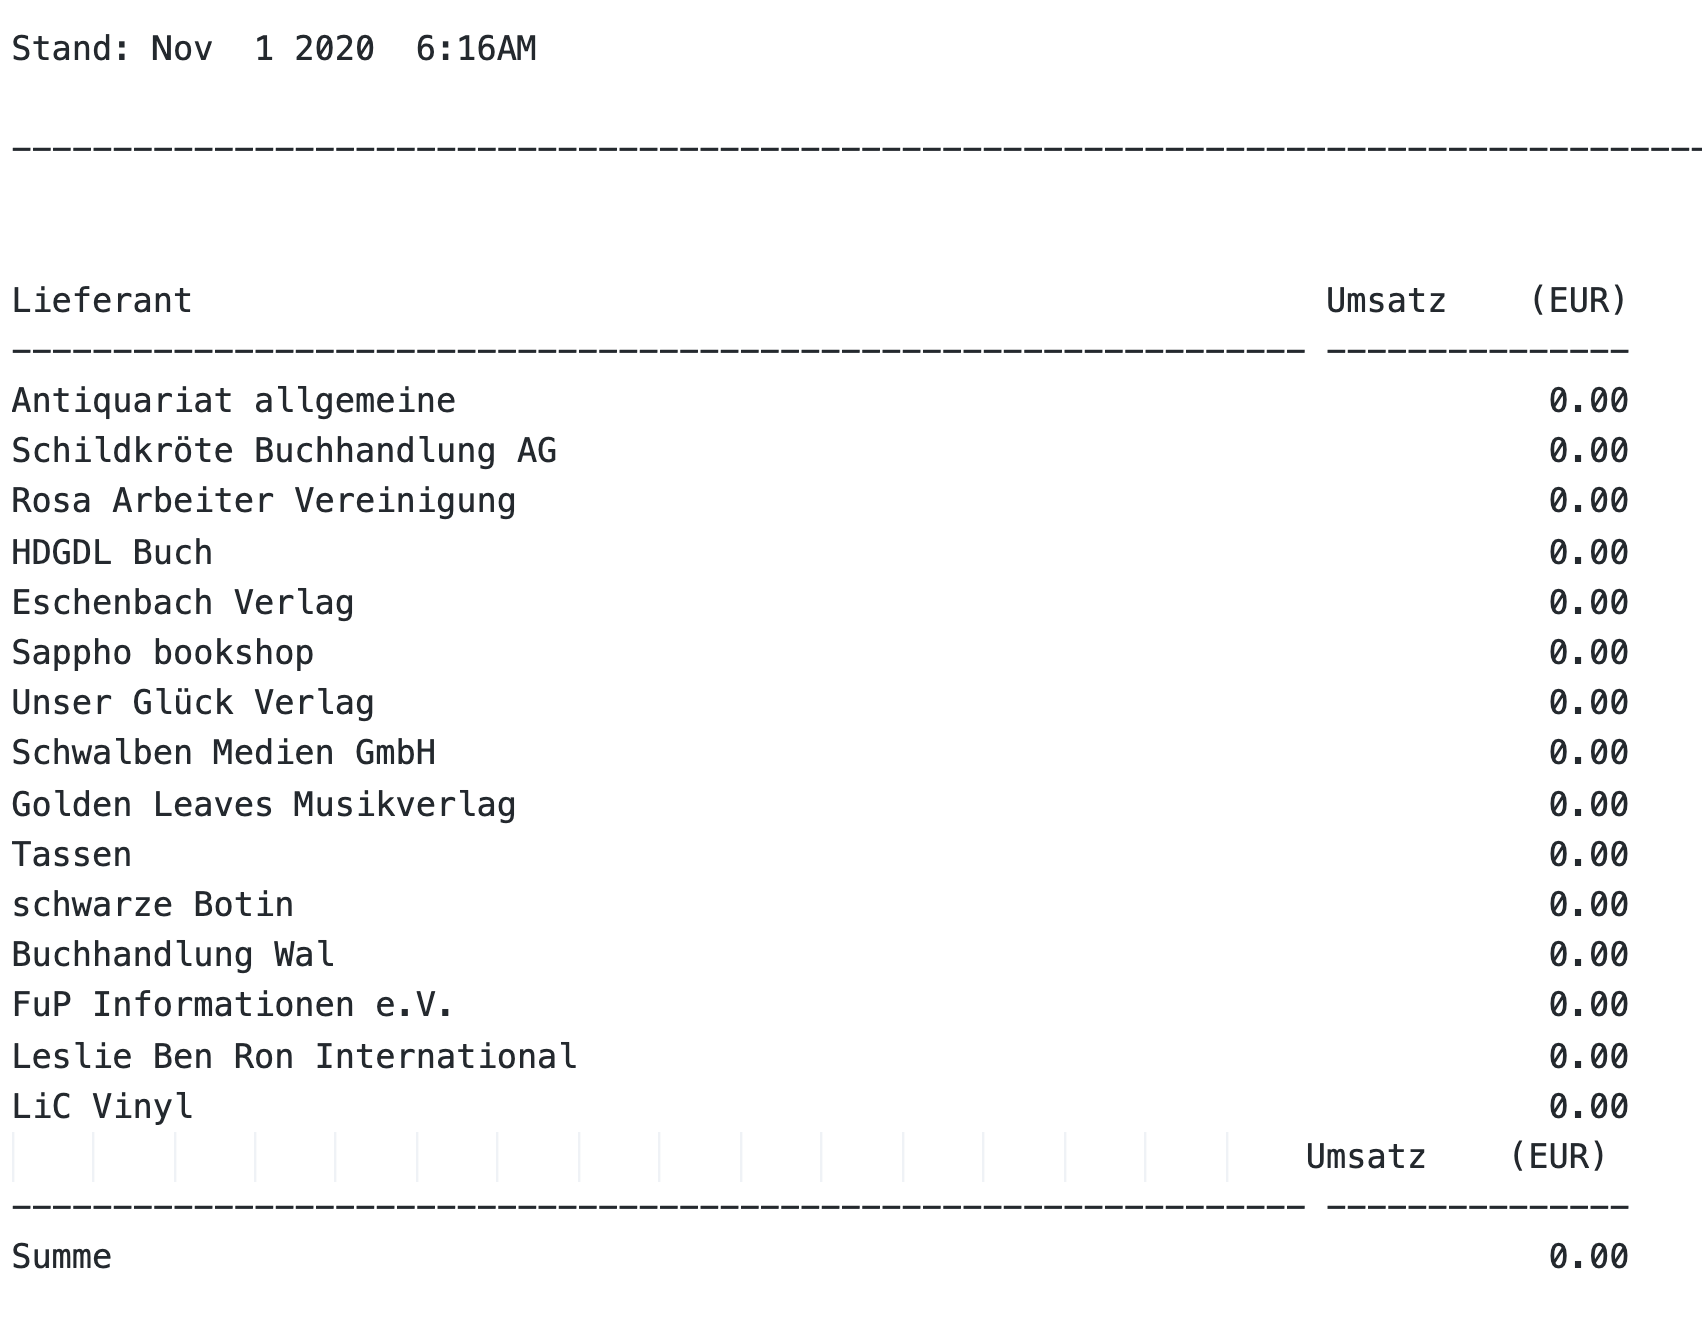
\includegraphics[width=8.5cm, height=9.0cm]{umsatz_mtl}
            %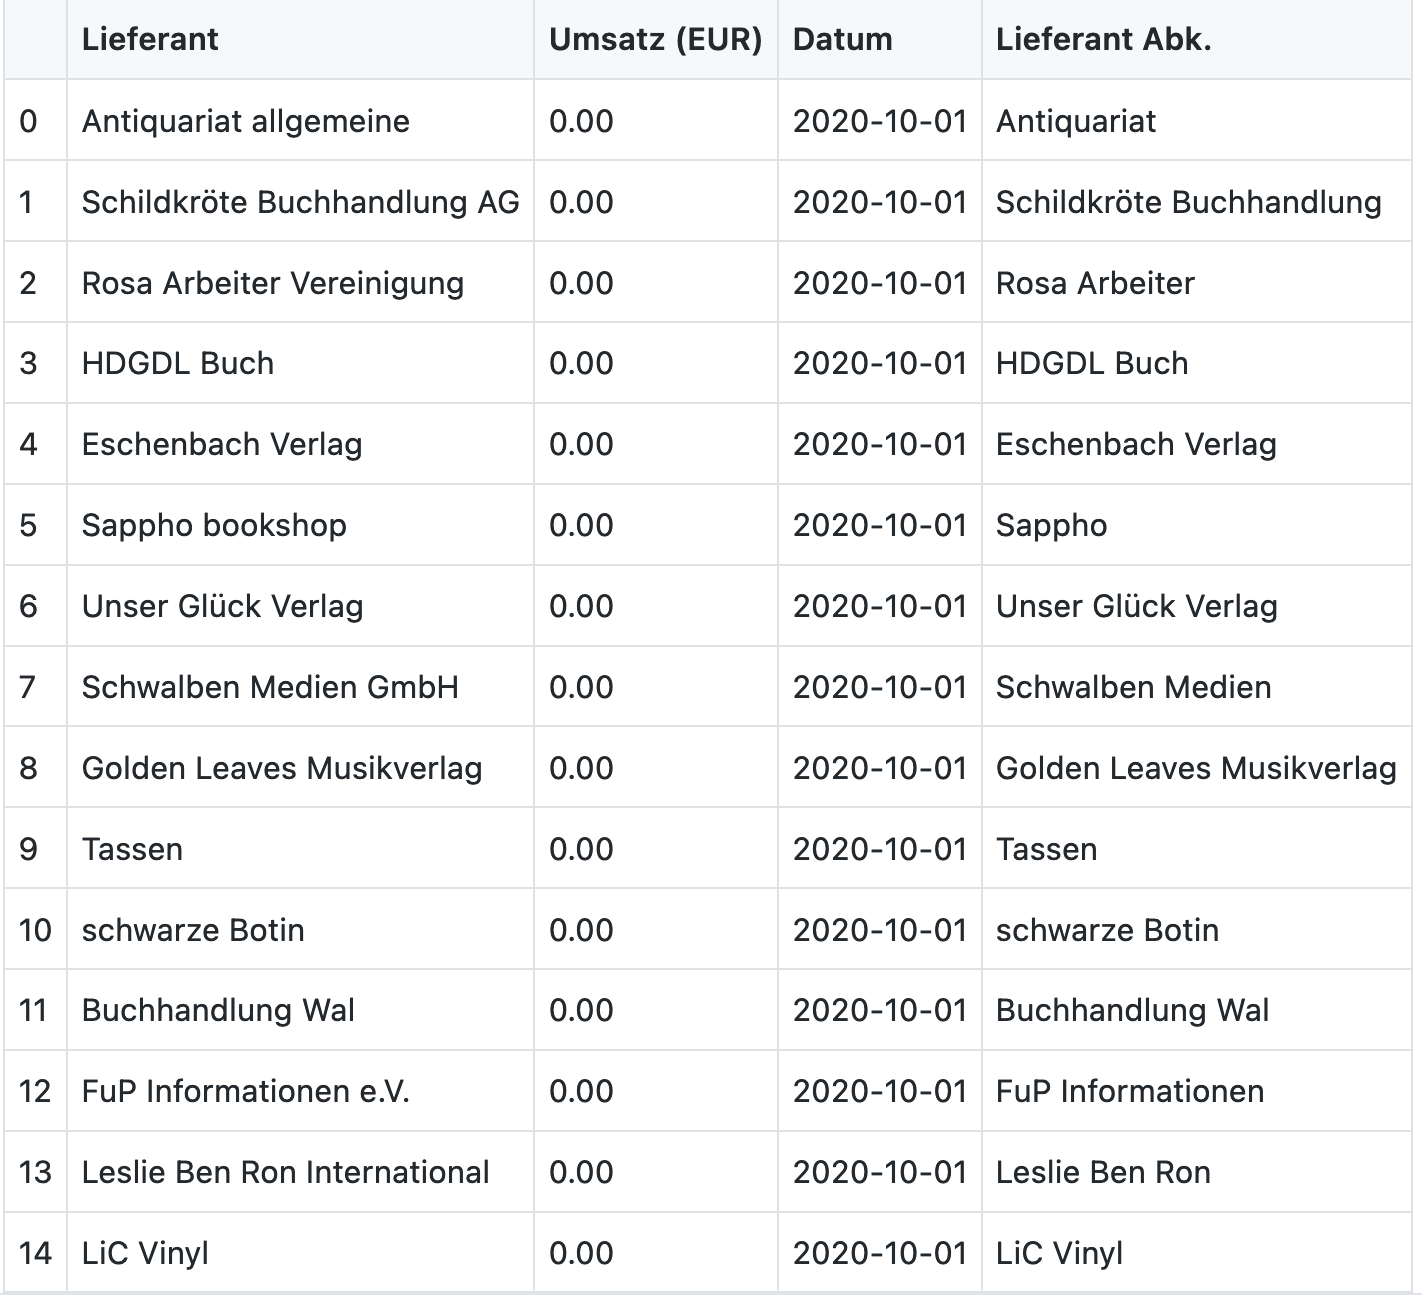
\includegraphics[width=6.5cm, height=7.0cm]{umsatz_csv}
            \caption{Monatliche Umsatzübersicht vor Ablauf Teilsystem 1 Import}
            \label{fig:umsatzuebersicht_txt}
    \end{figure}


    \begin{figure}[H]
        \centering
            %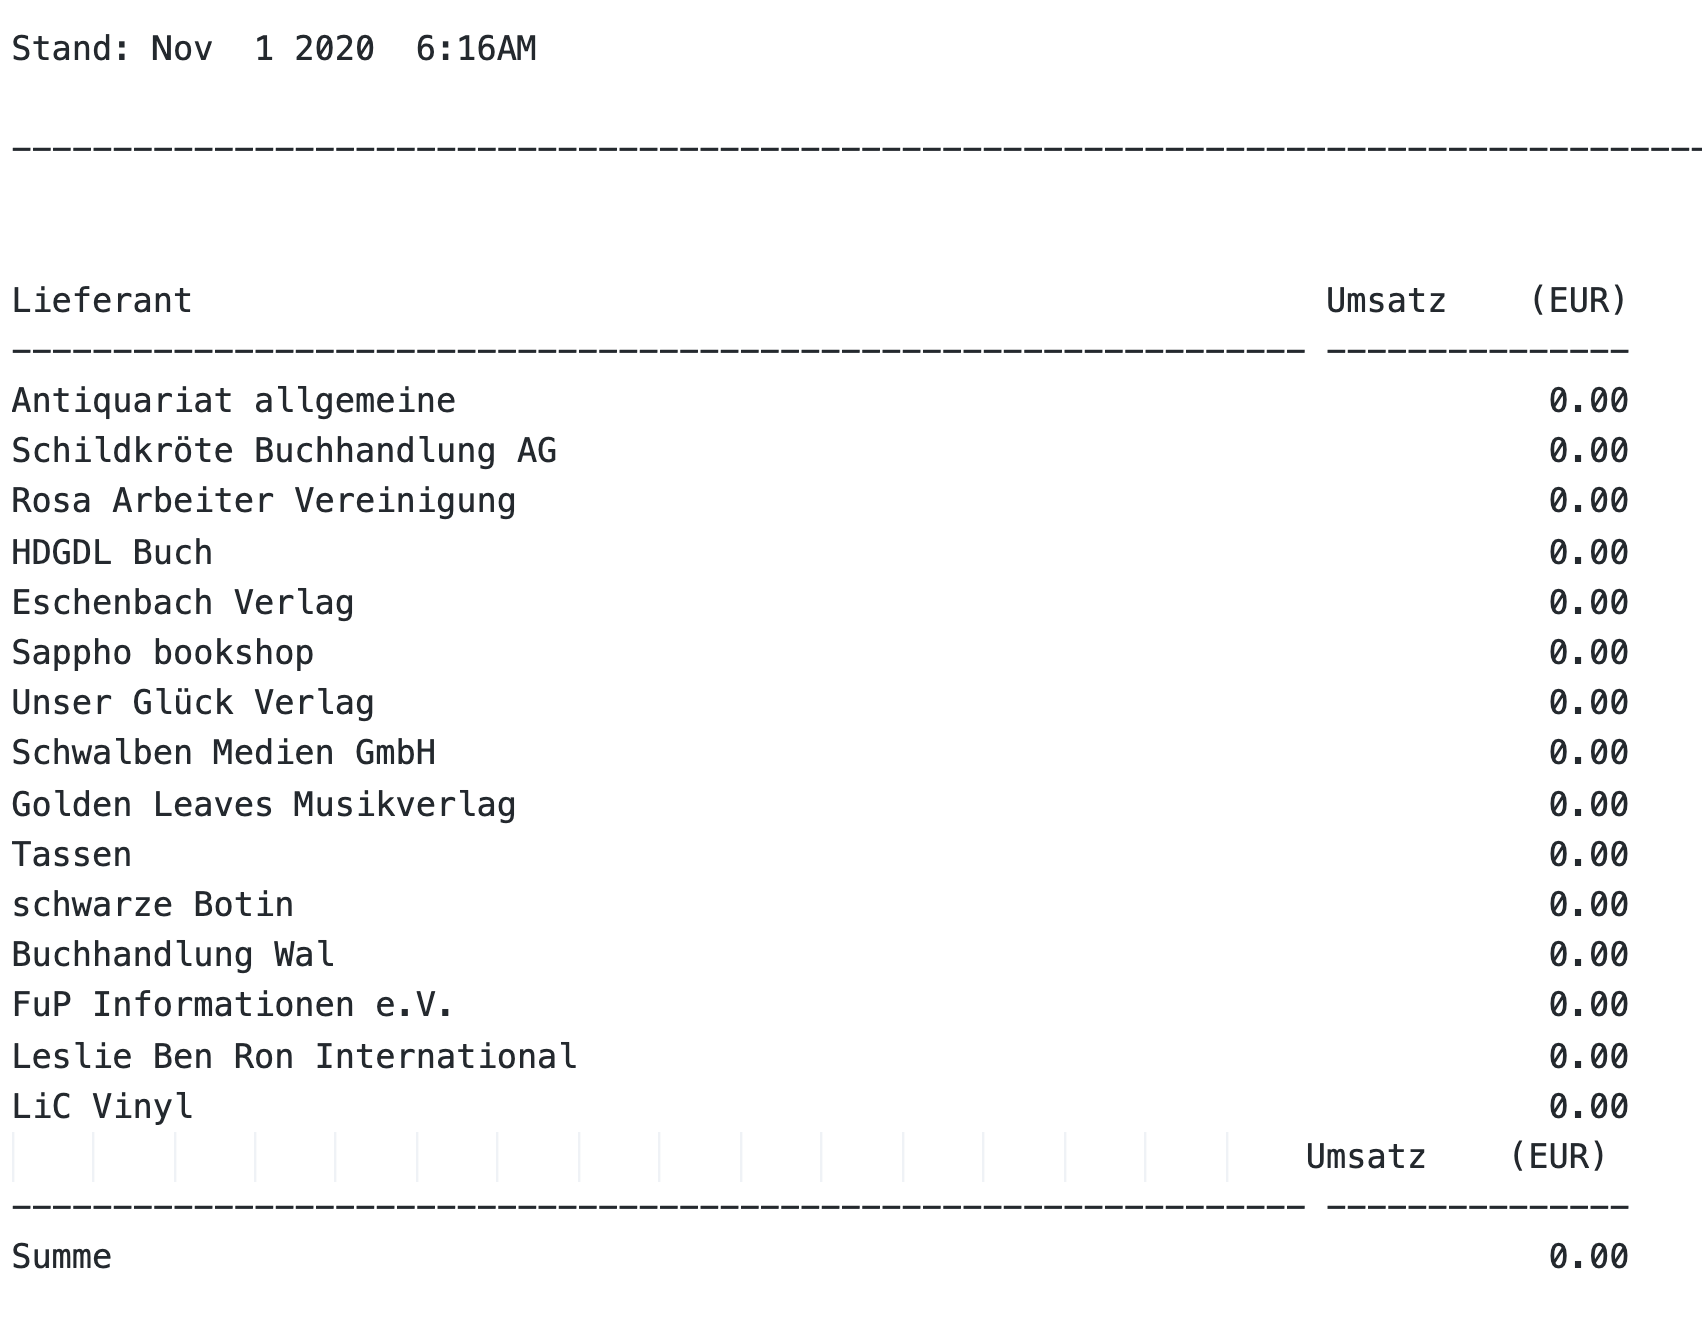
\includegraphics[width=6.5cm, height=7.0cm]{umsatz_mtl}
            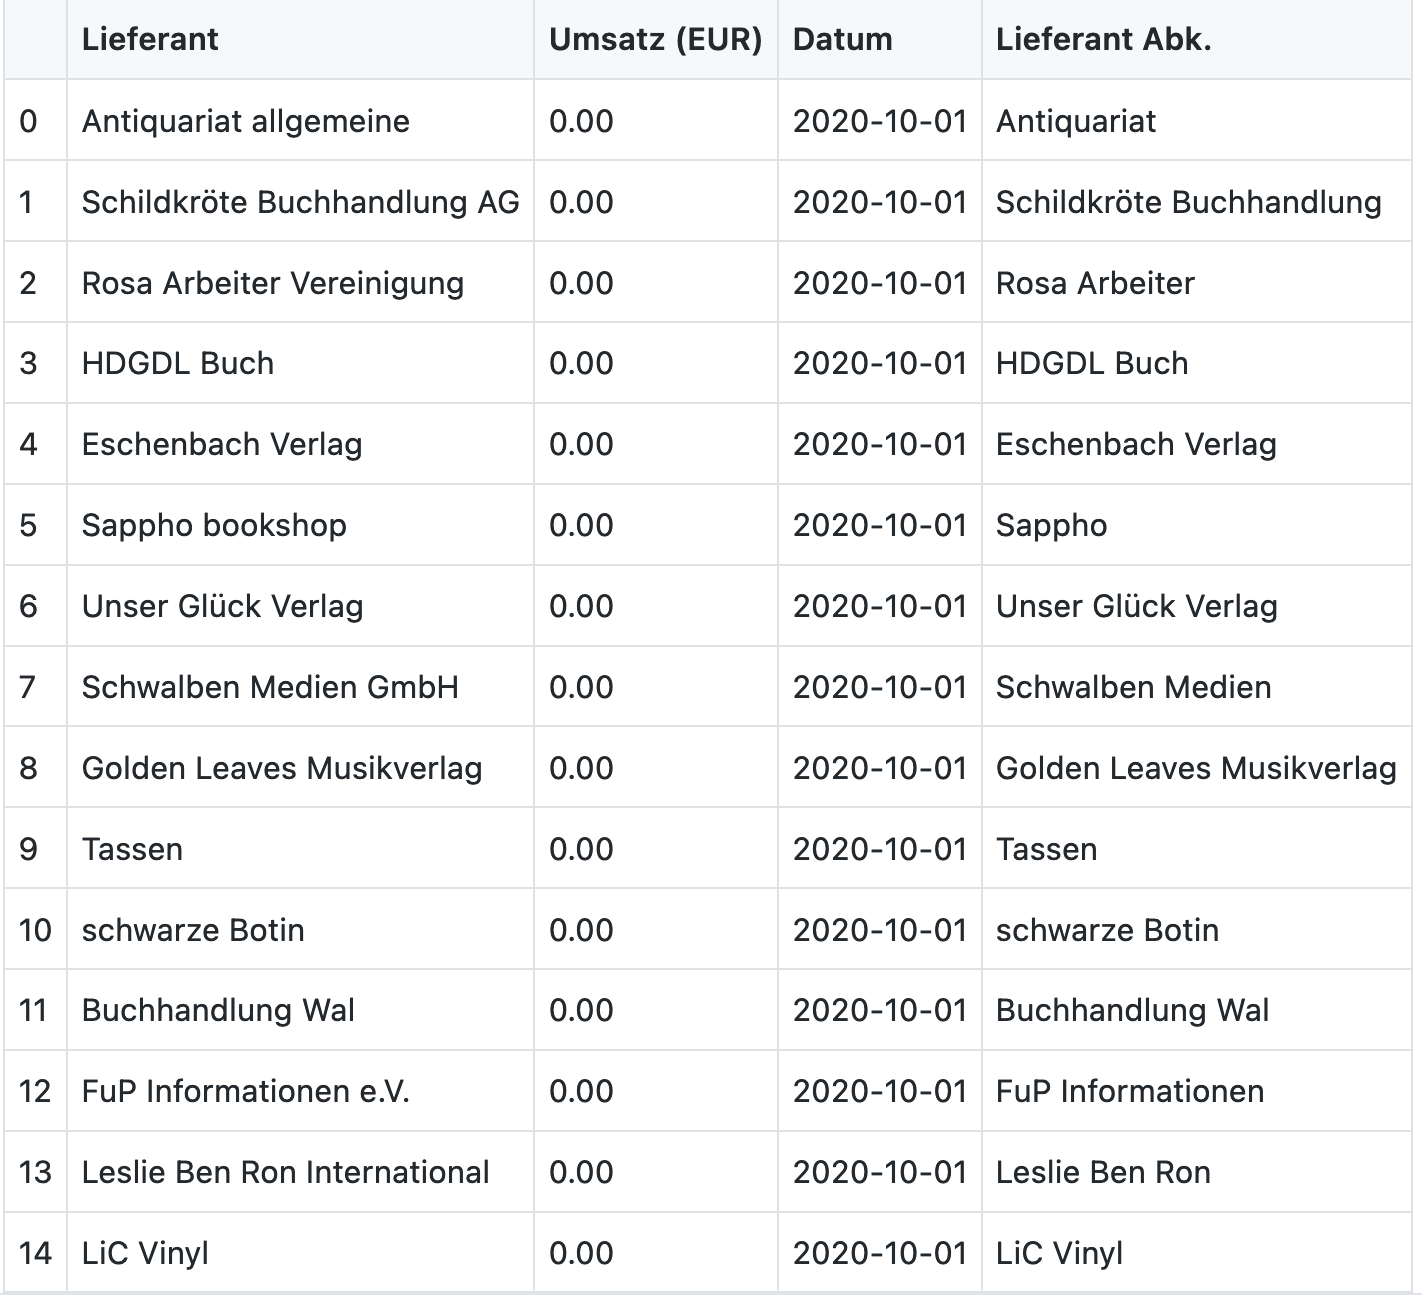
\includegraphics[width=8.5cm, height=9.0cm]{umsatz_csv}
            \caption{Monatliche Umsatzübersicht nach Ablauf Teilsystem 1 Import}
            \label{fig:umsatzuebersicht_csv}
    \end{figure}

    Die Daten liegen nun in den Speicherverzeichnissen vor und können nun durch das \textit{Teilsystem 2 Datenbearbeitung} 
    weiterbearbeitet werden.
    
    %\clearpage
    \noindent
    \textit{Teilsystem 2 Datenbearbeitung}

    \begin{figure}[H]
        \centering
            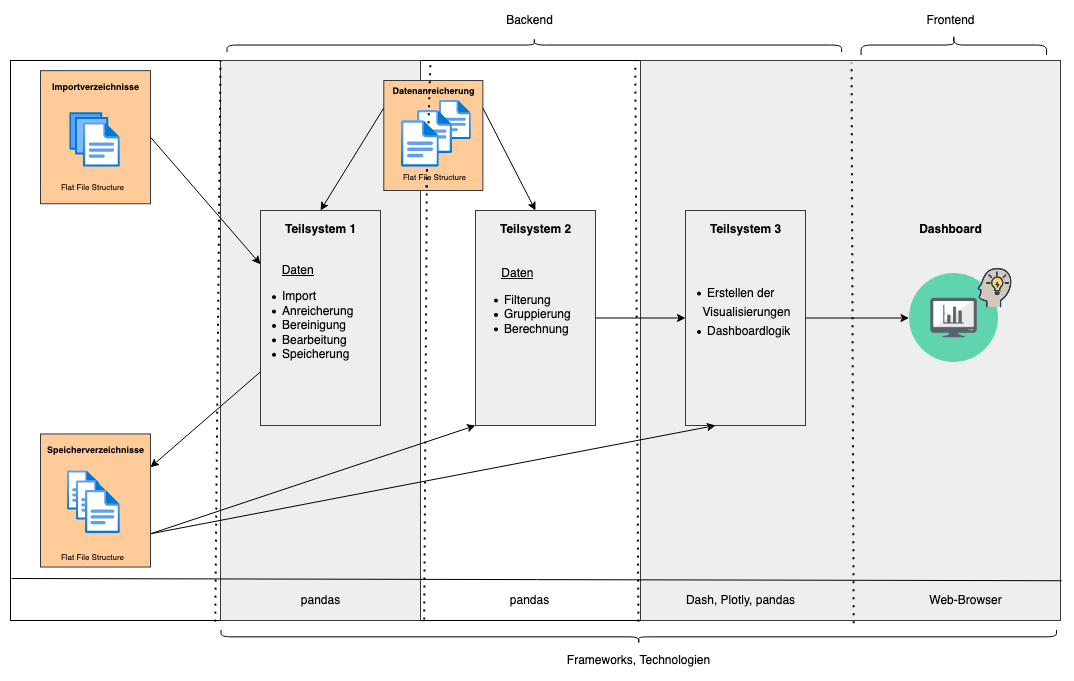
\includegraphics[width=15cm, height=10cm]{Systemarchitektur_Ts2}
            \caption{Systemarchitektur Teilsystem 2}
            \label{fig:Systemarchitektur Teilsystem 2}
    \end{figure}

    Das \textit{Teilsystem 2 Datenbearbeitung} hat das Ziel, die Daten für die Darstellung im Dashboard vorzubereiten. Der weitere Zweck dieses
    Teilsystem ist, die Vorbereitung der Daten von der Erstellung der Datenvisualisierungen zu trennen. Ein Grund hierfür
    ist, den Programmcode im Teilsystem 3 nicht mit dem Programmcode der Datenmanipulation zu überfrachten. Die  Berechnungen
    werden zur Laufzeit des Dashboards ausgeführt und somit im Hauptspeicher gehalten.
    Deswegen werden in dem Teilsystem Datenbearbeitung Daten mit pandas so bearbeitet, 
    dass entweder Teilmengen der eigentlichen Daten oder Ergebnisse mathematischer Operationen durch das Teilsystem 3 
    zu Datenvisualisierungen nur noch weiterverarbeitet werden müssen. Die Vorbereitung der Daten umfasst einzelne Berechnungen 
    wie \texttt{mean()} oder \texttt{sum()}. Ferner werden im Teilsystem 2 die Sortierung, Gruppierung und Filterung der 
    Daten nach bestimmten Aspekten vollzogen, die in den Anwendungsfällen im \autoref{chap:four_one_five} formuliert sind.
    
    Für das \textit{Teilsystem 2 Datenbearbeitung} ist das Modul \texttt{data\_prep} zentral. Die Klassenstruktur dieses Moduls ist eine 
    Basisklasse, von der vier Kindklassen erben. Es gibt Kindklassen für Umsatz- und Budgetdaten, für Bestands- und Neuerwerbungsdaten sowie für die Daten der Ausleihe und 
    der Lesesaalnutzung. Aufgrund der ähnlichen Datenstruktur der Umsatz- und Budgetdaten genügt eine Klasse für beide.
    Der Gesamtbestand und die monatlichen Neuerwerbungen berufen sich auf denselben Datenbestand, sodass hier ebenfalls auf eine Aufteilung auf mehrere Klassen verzichtet wurde.
    Für jede Kindklasse wurden Methoden geschrieben, die auf den spezifischen Bibliotheksdaten verschiedene Manipulationen ausführen.
    Die Ergebnisse werden von jeder Methode zurückgeben. \autoref{fig:classes data_prep} zeigt die Basisklasse und die vier Kindklassen mit ihren Methoden.

    \begin{sidewaysfigure}

    %\begin{figure}[H]
        \centering
            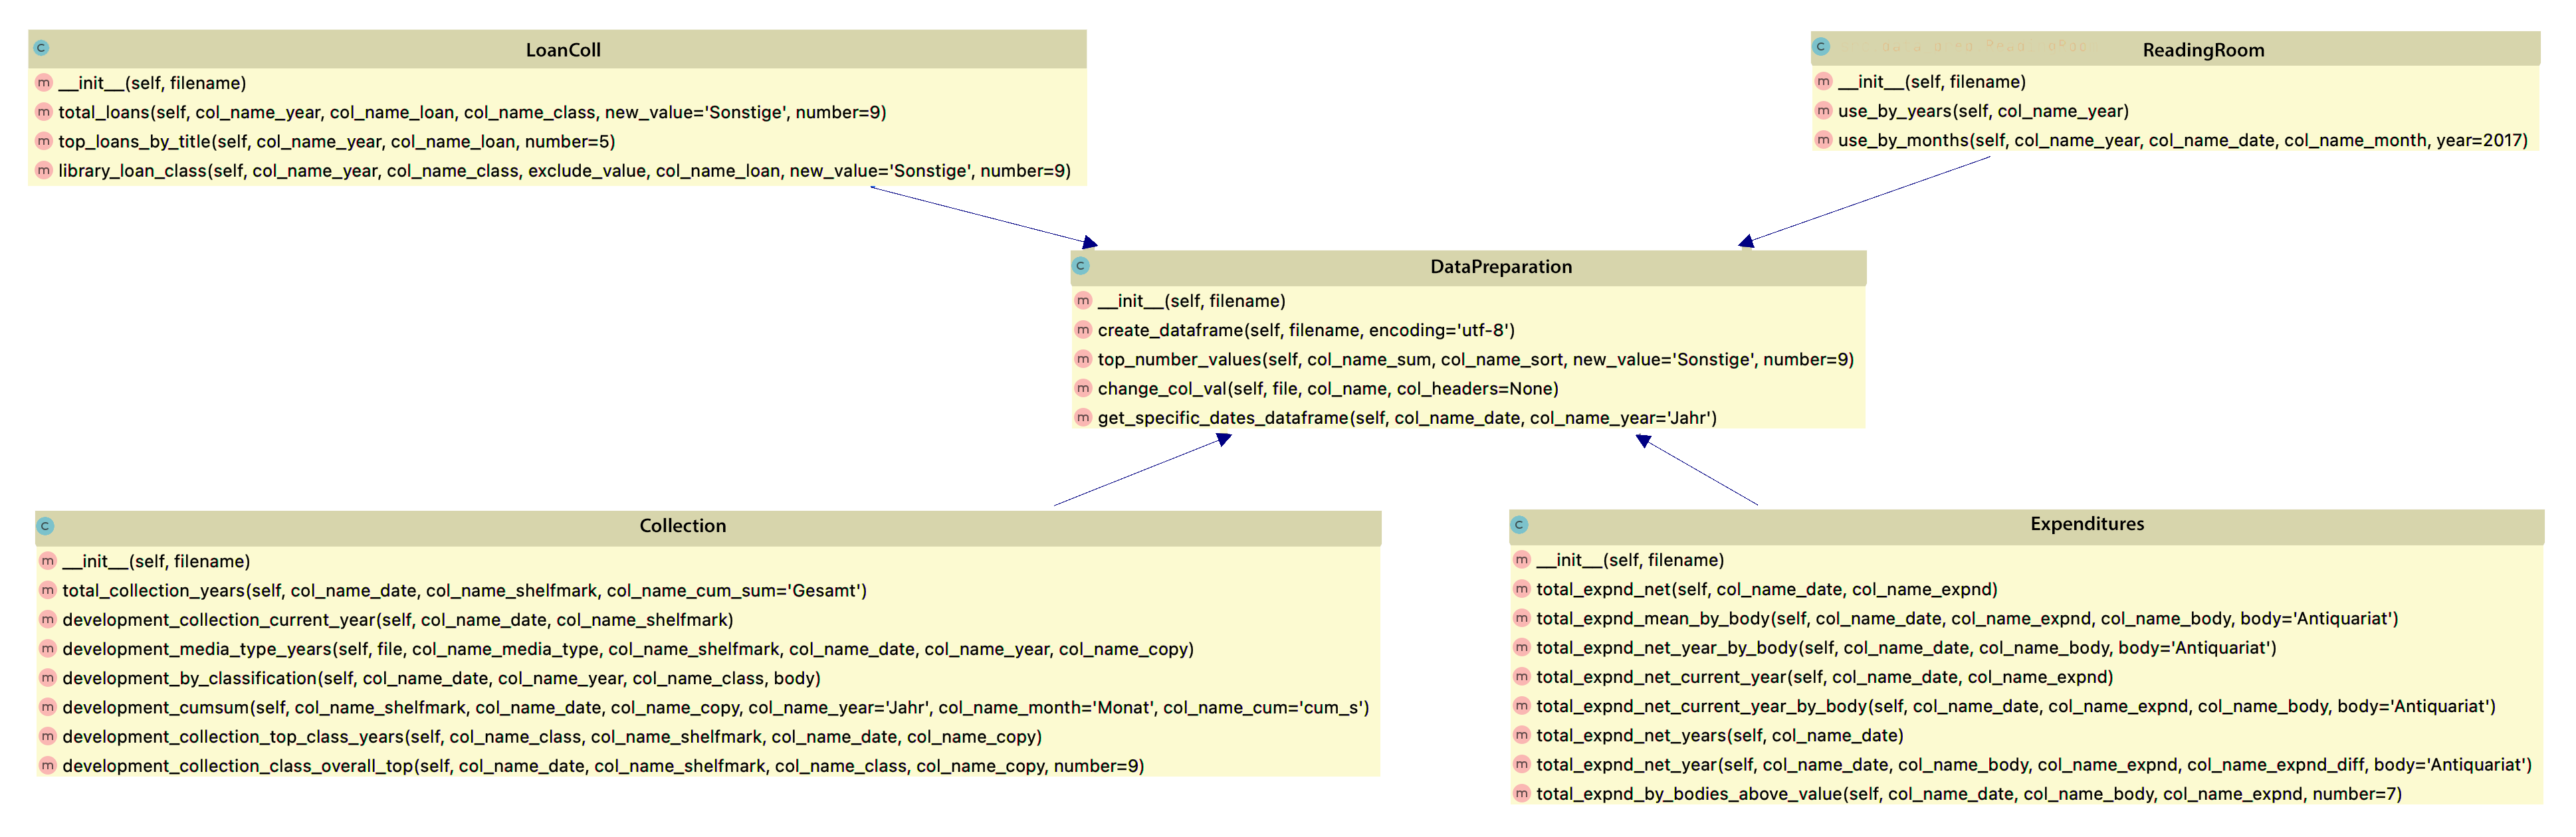
\includegraphics[width=21.5cm, height=12cm]{data_prep_class}
            \caption{Klassendiagramm - Teilsystem 2 Datenbearbeitung}
            \label{fig:classes data_prep}
    \end{sidewaysfigure}
    %\end{figure}

    Der Ablauf innerhalb des Teilsystems besteht aus zwei Schritten.\\
    (1) Das Laden der einzelnen csv-Dateien in dem pandas Dataframe aus dem Zielverzeichnis wird durch die Methode \texttt{create\_dataframe()} der Basisklasse geregelt.
    %Es wird noch einmal sichergestellt, dass die Daten in einem Zeichenformat wie utf-8 in das pandas Dataframe geladen werden.
    Beim Aufrufen des Konstruktors beziehungsweise der \texttt{init}-Methode der Klasse wird die Methode \texttt{create\_dataframe()} 
    automatisch mit aufgerufen. In den Kindklassen wird ebenfalls das Objekt mit dem pandas Dataframe instantiiert, da die Konstruktor-Properties der Basisklasse 
    an die Kindklassen mitvererbt werden. Die Objekte können nach Instantiierung durch die spezifischen Methoden der Kindklassen bearbeitet werden.
    
    (2) Das Ergebnis der Manipulation der pandas Dataframes ist auf die Darstellung der Daten im Dashboard ausgerichtet. Als Input der einzelnen Methoden der
    Kindklassen werden verschiedene Parameter verlangt, mit deren Hilfe der Dataframe entweder manipuliert wird oder auf ihm Berechnungen ausgeführt werden können. 
    Um die Daten für das Teilsystem 3 vorzubereiten, können verschiedene Transformationsschritte auf den Daten in den Methoden ausgeführt werden. 
    Die Rückgabewerte der Methoden sind veränderte pandas Dataframes, pandas Series oder einzelne Skalare mathematischer Operationen.
    
    % Bei der folgenden Methode interessieren für die Darstellung im Dashboard nur die Umsatz/Budget-Daten für spezifische Datums-Daten. Hintergrund ist der, dass die 
    % monatlichen Umsatz- und Budgetdaten im Jahr akkumuliert werden. Wenn das Budget und der Umsatz nur Jahresweise dargestellt werden sollen, 
    % interessieren dementsprechend nur die Datensätze jeweils vom Dezember beziehungsweise vom aktuellen Monat im Jahr.
    

    % \begin{lstlisting}[language=Python, caption=Python example]
        
    %     def total_expnd_net_years(self, col_name_date):
    %         ...
    %         self._df = self.get_specific_dates_dataframe(col_name_date)
    %         return self._df

    % \end{lstlisting}
    

    % Die Methode \texttt{total\_expnd\_net\_years} der \texttt{Expenditures}-Klasse gibt nach einem Transformationsschritt einen pandas Dataframe zurück.
    % Der Transformationsschritt beinhaltet die Filterung des Dataframes nach spezifischen Werten in der Spalte des übergebenden Spaltennamens.
    % Zu diesem Zweck wird noch die Methode\\
    % \texttt{get\_specific\_dates\_dataframe} aufgerufen. 
    Anhand der folgenden Methode \texttt{total\_expnd\_net\_current\_year()} soll der letzte Schritt verdeutlicht werden.
    Die Methode der \texttt{Expenditures}-Klasse bestimmt im Allgemeinen die Summe von Werten einer Spalte, gefiltert
    nach einem Wert einer anderen Spalte eines pandas Dataframes. Mit dieser Methode soll so zum Beispiel konkret der Gesamtumsatz des 
    laufenden Jahres bestimmt werden.

    \begin{lstlisting}[language=Python, caption=Beispiel Methode Expenditures class]
    def total_expnd_net_current_year(self, col_name_date, col_name_expnd):
        ... 
        date_max = self._df[col_name_date].max()        
        self._df = self._df.set_index(col_name_date)
        self._df = self._df.loc[date_max]

        return self._df[col_name_expnd].sum()  
    \end{lstlisting}

    Als Input erwartet die Methode in der Methodensignatur zwei Spaltennamen als Parameter: den Namen der Datumspalte \texttt{col\_name\_date}, nach der gefiltert wird,
    und den Namen der Umsatz-Spalte \texttt{col\_name\_expnd}, auf der die Berechnung stattfindet. Der Transformationsprozess im Methodenkörper teilt sich in drei Schritte auf. Da die monatlichen Umsatzdaten im Jahr als 
    akkumulierte Daten vorliegen, interessieren nur die Datensätze mit dem größten Datumswert. Deswegen
    wird nach diesen gefiltert und ein Dataframe von diesen erstellt. Dementsprechend wird mit der pandas-Funktion \texttt{max()} 
    zunächst der maximale Wert in der Datumsspalte bestimmt und der Variable \texttt{date\_max} zugewiesen. Danach wird die Datumsspalte als Index gesetzt. 
    Im dritten Schritt wird der Dataframe mit den Reihen, die der Variable \texttt{date\_max} entsprechen, erstellt. Dies geschieht mit der pandas-Funktion \texttt{.loc}, die
    auf den Index der Reihen des Dataframes zugreift. Zum Schluss wird auf Basis der Umsatz-Spalte des Dataframes die Summe mit der pandas-Funktion \texttt{sum()} berechnet 
    und als Rückgabewert zurückgeliefert. Der Rückgabewert kann nun vom \textit{Teilsystem 3 Darstellung} weiterverarbeitet werden.\\

    \noindent
    \textit{Teilsystem 3 Darstellung}\\

    \begin{figure}[H]
        \centering
            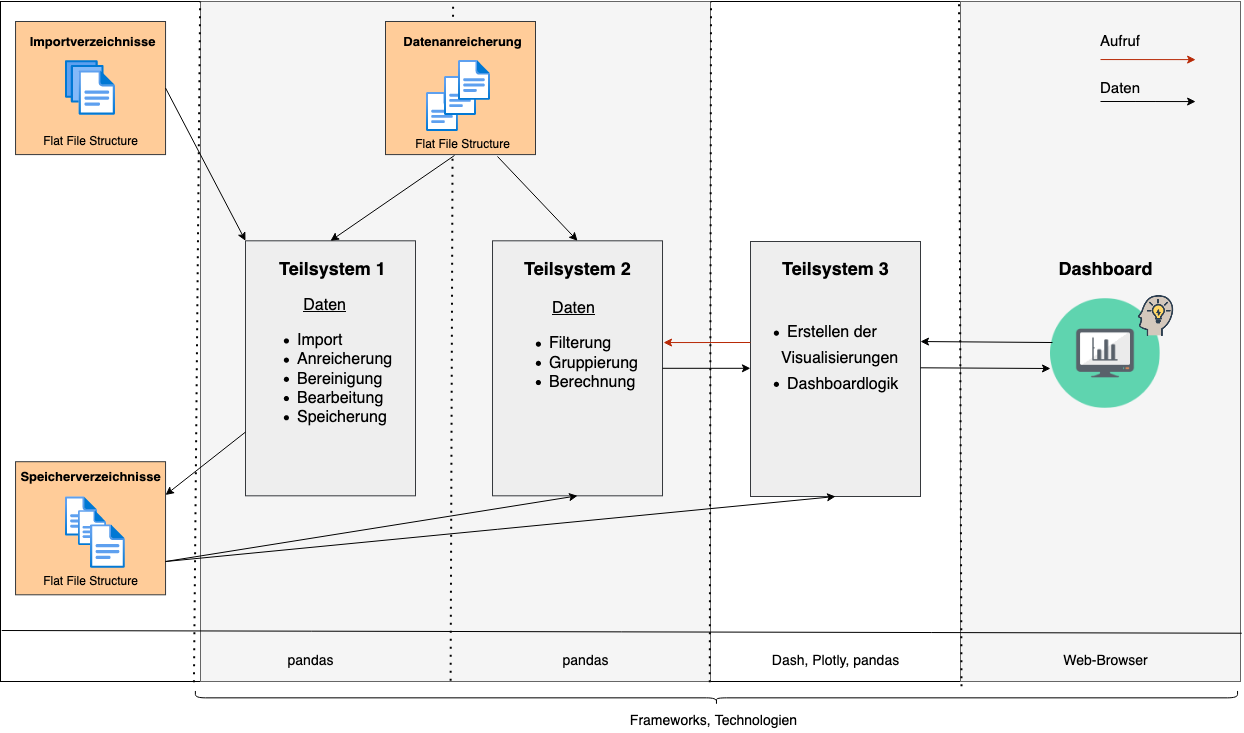
\includegraphics[width=15cm, height=10cm]{Systemarchitektur_Ts3}
            \caption{Systemarchitektur Teilsystem 3}
            \label{fig:Systemarchitektur Teilsystem 3}
    \end{figure}

    Für die Erschaffung des Dashboards mit seinen Datenvisualisierungen und Interaktionen ist das \textit{Teilsystem 3 Darstellung} verantwortlich.
    In ihm werden die Ergebnisse des Teilsystems 2 zu Datenvisualisierungen verarbeitet und die Dashboard-Logik bereitgestellt.
    Die Übergabe der Daten erfolgt durch den Aufruf der Objekte und der Methoden aus den Kindklassen des \texttt{data\_prep}-Moduls aus dem Teilsystem 2.
    %In ihm werden die Datenvisualisierungen mit den den Ergebnissen aus dem Teilsystem Datenbearbeitung
    %geschaffen. 
    Die Bibliothek Plotly Express  wird für die Datenvisualisierungen und die Bibliothek Dash zur Umsetzung des Dashboards genutzt. 
    
    Die Struktur der Dashboard-App entspricht einem Multi-App-Dashboard.
    Aufgrund der Vielzahl an Datenvisualisierungen wurde sich gegen eine Single-Page-Lösung entschieden. Deswegen besteht das Dashboard
    aus drei einzelnen Tabs, auf die die einzelnen Datenvisualisierungen aufgeteilt sind.
    % Aufgrund der vielen Code-Blöcke tendieren Dashboards-Apps, die mit Dash geschrieben wurden zur Unübersichtlichkeit.
    
    Es gibt verschiedene Möglichkeiten Multi-App-Dashboard-Projekte zu strukturieren. Für das vorliegende Projekt wurde sich für die in 
    \autoref{fig:dash structure} gezeigte Struktur entschieden.

    \begin{figure}[H]
        \centering
            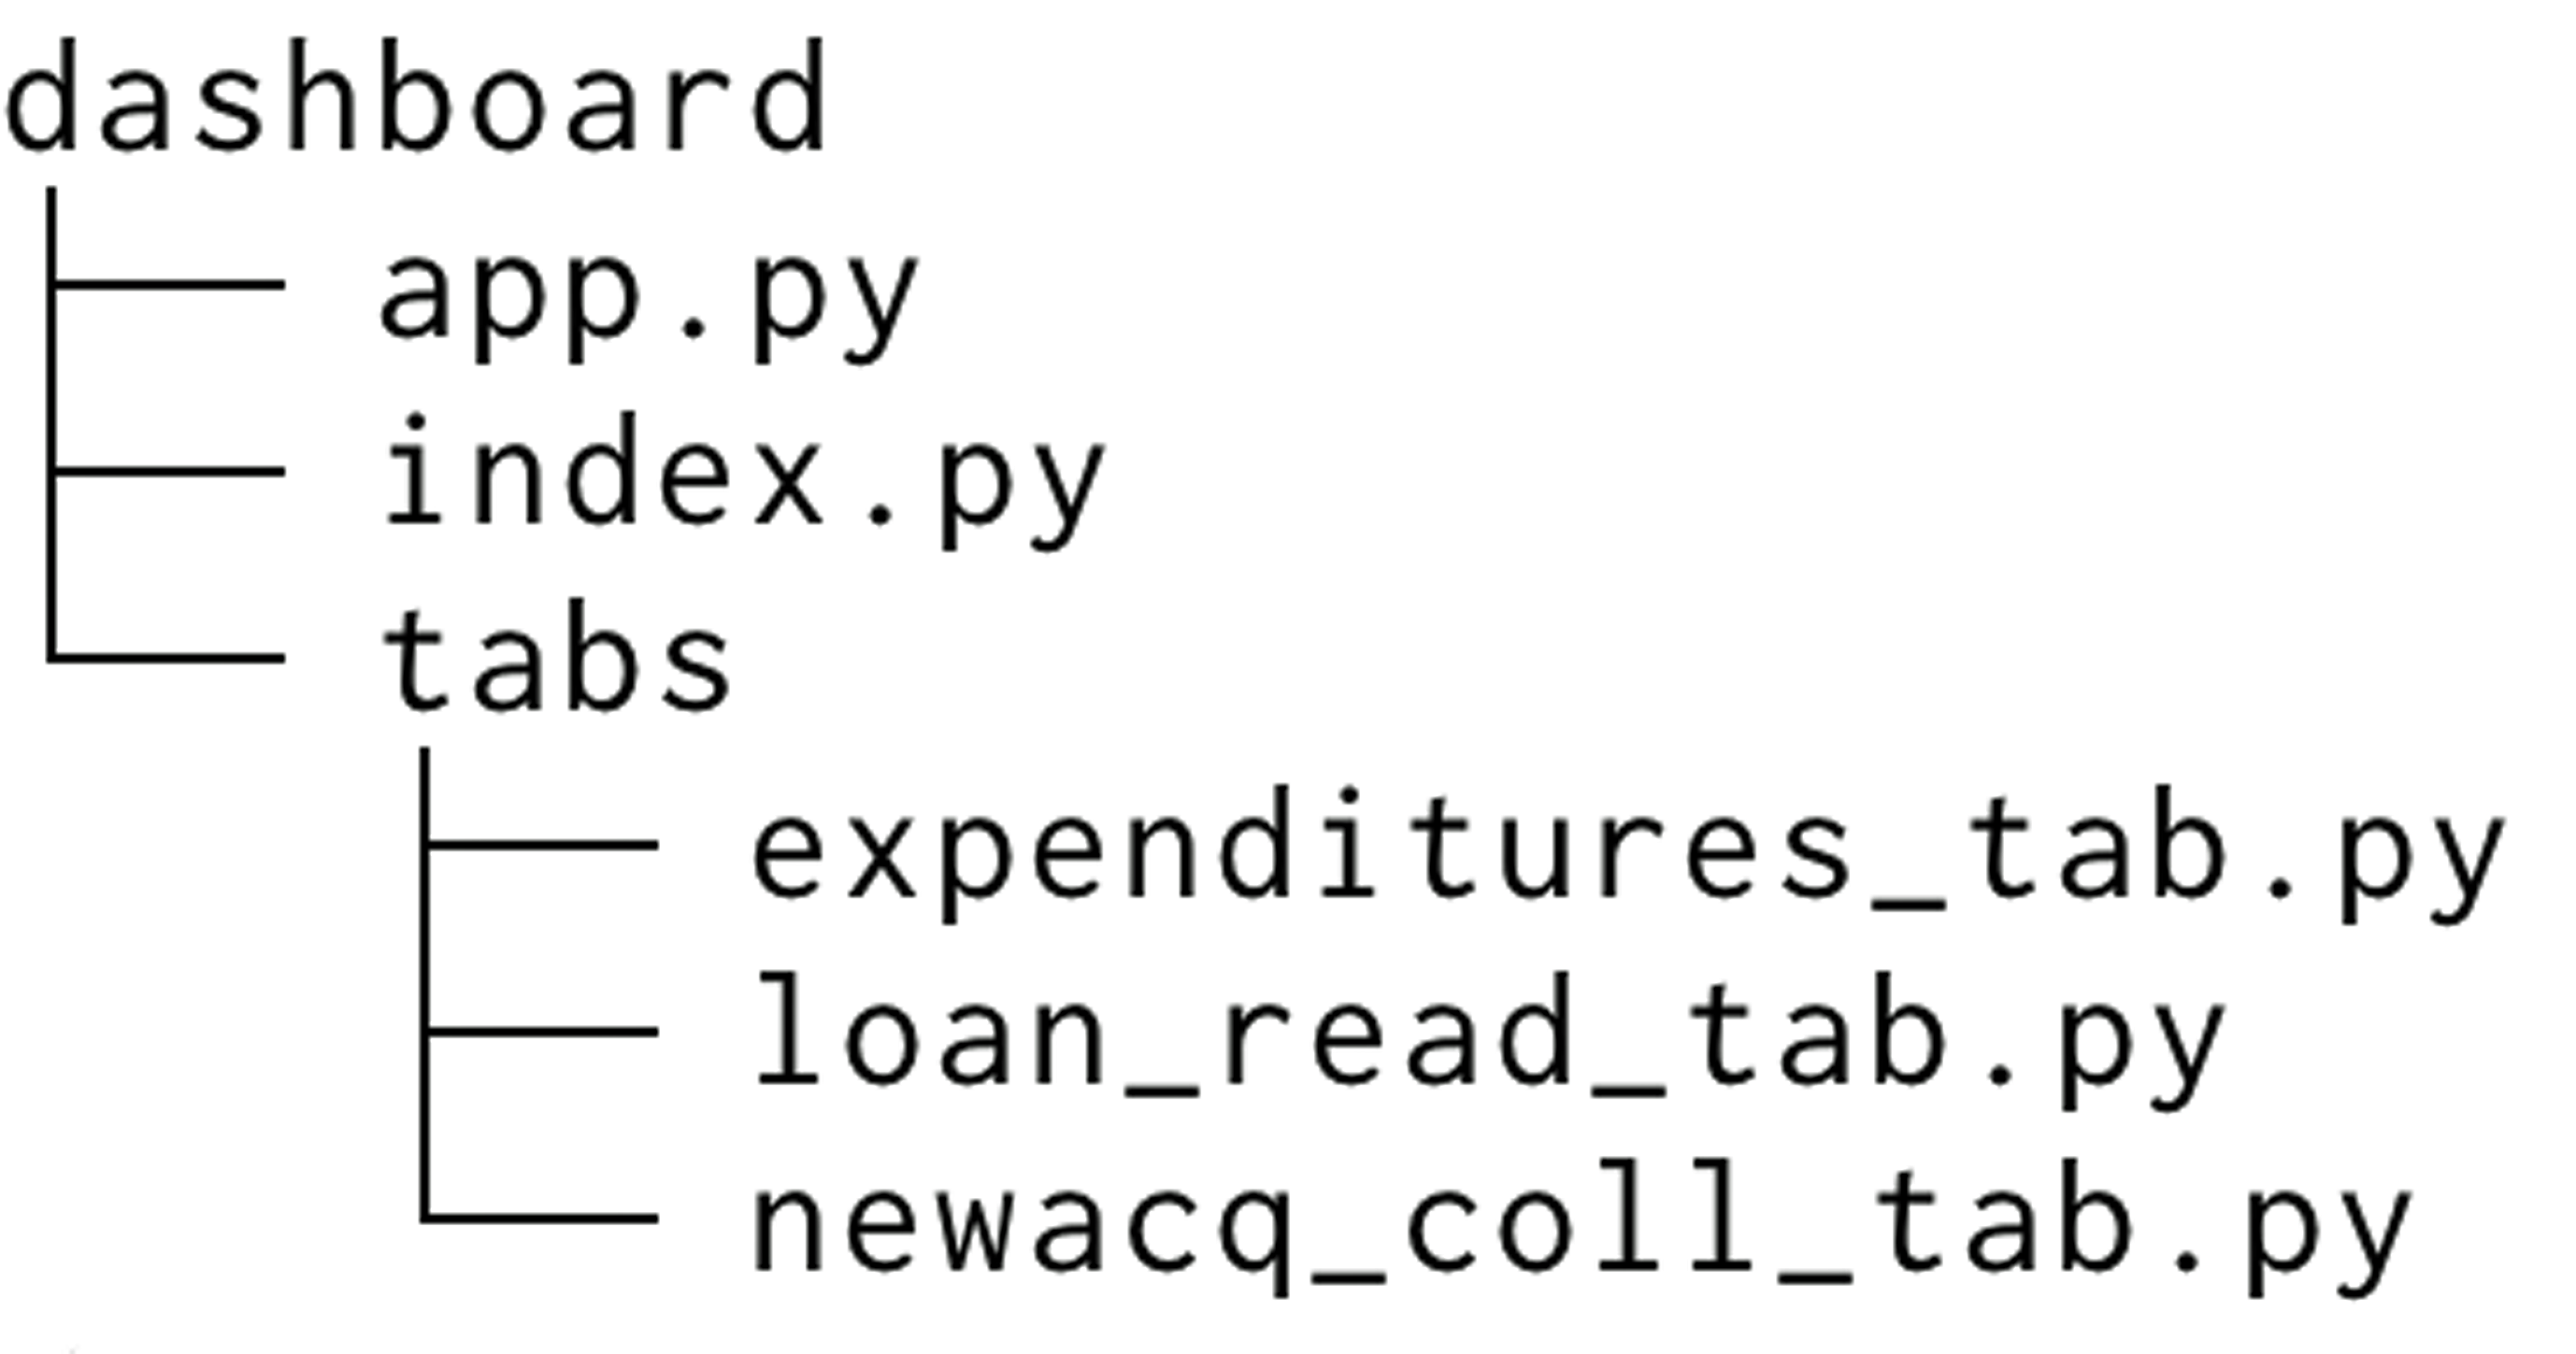
\includegraphics[width=6cm, height=3.5cm]{dash_struc}
            \caption{Struktur Dash Multi-Page App}
            \label{fig:dash structure}
    \end{figure}
    
    Dies ist eine Möglichkeit, wie sie auf der Webseite von Dash für Multi-App-Projekte vorgeschlagen wird \cite[vgl.][]{plotly_url_2021}.
    
    Die einzelnen Tabs wurden inhaltlich um bibliothekarische Tätigkeiten zu gruppieren. So werden in der \texttt{expenditures\_app.py}
    Datenvisualisierungen erstellt, die Budget- und die Umsatzdaten visualisieren, während mit Hilfe der \texttt{loan\_read\_app.py}
    Ausleih- und Lesesaalnutzungsdaten dargestellt werden. Mit der \texttt{newacq\_coll\_app.py} wird ermöglicht, Daten aus dem Bereich der Bestandsentwicklung und der 
    Ausleihe zu präsentieren.

    Für jeden Tab gibt es eine separate Datei. Jede einzelne Tab-Datei besteht einerseits aus mehreren Funktionen für die Erschaffung von Datenvisualisierungen der
    Ergebnisse aus Teilsystem 2.\footnote{Zur besseren Lesbarkeit heißt die Gruppe dieser Funktionen im Folgenden \texttt{fig\_()}.}
    Innerhalb dieser Funktionen werden mit den Plotly-Funktionen Plotly Graph Object Figures geschaffen. 
    Andererseits bestehen die Dateien aus mehreren verschiedenen Funktionen für die Dash-Komponenten wie zum Beispiel Dropdown-Menüs, Cards oder Diagrammen.\footnote{Ebenfalls zur besseren Lesbarkeit
    heißt die Gruppe dieser Funktionen im Folgenden \texttt{html\_()}.}
    Diese Funktionen binden die \texttt{fig\_()}-Funktionen so ein, dass die Plotly Graph Object Figures im Dashboard zur Anzeige gebracht werden können. 
    Weiterhin sind die \texttt{html\_()}-Funktionen zum Teil mit Dekorator-Callback-Funktionen verknüpft, die es ermöglichen, mit dem Dashboard zu interagieren. 
    Ferner enthalten die Dateien jeweils eine Layoutfunktion, die das gesamte Layout des Tabs bündelt.

    Neben den Funktionen für die Dash-Komponenten und der Datenvisualisierungen, werden in den tab-Dateien noch die benötigten Objekte aus dem Modul \texttt{data\_prep} 
    instantiiert und die Methoden der Kindklassen aus diesem Modul auf diesen angewendet. In der Regel geschieht dies außerhalb der Funktionen am Anfang 
    jeder Tab-Datei nach den Import-Anweisungen für die einzelnen Module. Für die Callback-Funktionalität werden aber die Objekte und die Methoden des Moduls \texttt{data\_prep} innerhalb einiger \texttt{html\_()} aufgerufen.
    Anhand der Erstellung von Plotly Graph Object Figures wird exemplarisch auf den Aufbau und die Funktionsweise der Funktionen in den Tab-Dateien im Folgenden näher eingegangen.
    \footnote{Auf die Erzeugung von anderen Dash-Elementen wie Cards wird dabei aufgrund der Übersichtlichkeit der Darstellung nicht Bezug genommen. Diesem liegt ein ähnlicher Prozess
    zu Grunde. Es werden aus den berechneten Ergebnissen der Objekte direkt Dash-Komponenten mit Hilfe der \texttt{dash\_bootstrap\_components} erstellt.}
    
    Schematisch zeigt die \autoref{fig:process tab} die Ablauflogik in den Tab-Dateien ohne die callback-Funktionen.
    Die Objekte werden zunächst in Plotly Graph Objects umgewandelt. Diese wiederum werden in Dash-Objekte transformiert und diese werden 
    letztlich in einem Tab-Layout zusammengefasst.
    
    \begin{figure}[H]
        \centering
            \includegraphics[width=12cm, height=16 cm]{ablauf_tab_ps}
            %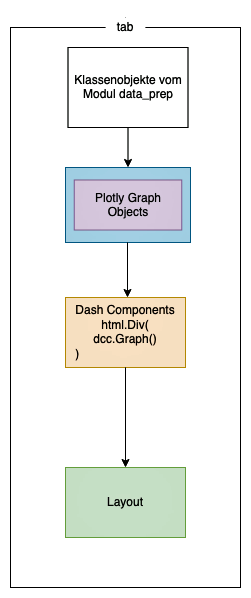
\includegraphics[width=6cm, height=8cm]{ablauf_dash_ohne_cb}
            \caption{Ablauf Tab}
            \label{fig:process tab}
    \end{figure}

    % Die grundsätzliche Logik der Funktionsaufrufe sieht in den Tab-Dateien ohne die Callback-Funktionen wie folgt aus:
    Die Erstellung der Diagramme und die Implementierung der Dashboard-Logik erfolgt durch ein nacheinander aufrufen von Funktionen.



    % \begin{figure}[H]
    %     \centering
    %         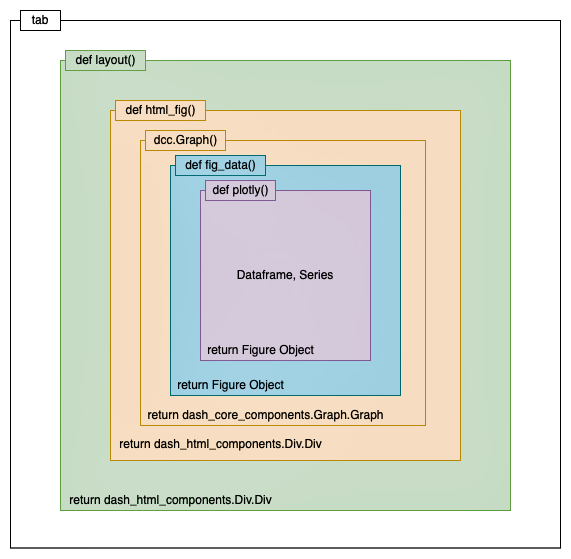
\includegraphics[width=10cm, height=8cm]{funktions_aufrufe_tab}
    %         \caption{Funktionsaufrufe Tab}
    %         \label{fig:function call tab}
    % \end{figure}

    In der Plotly-Funktion, die das Plotly Graph Object Figure erzeugt, werden die durch die Methoden der Kindklassen bearbeiteten Objekte (Dataframes, Series) 
    als Parameter entgegengenommen. Zusätzlich müssen noch weitere Parameter übergeben werden, die für die jeweiligen Diagrammtypen wichtig sind.
    Andere Parameter, die das Layout festlegen, sind dagegen optional \cite[vgl.][]{plotly_plotlygraph_objectsbar_2021}.
    
    Im folgenden Beispiel wird in der Funktion \texttt{fig\_total\_expnd()} aus \texttt{expenditures\_app.py} ein horizontal gekipptes Figure-Objekt
    mit dem pandas Dataframe \texttt{df\_total\_expnd} durch den Aufruf der Plotly-Funktion \texttt{bar()} erstellt. 
    Es werden zusätzlich in dem Funktionsaufruf noch die x-Achse und y-Achse mit den Werten der Spalten \enquote{Umsatz (EUR)} und \enquote{Datum} festgelegt. 

    \begin{lstlisting}[language=Python, caption=Funktion fig\_total\_expnd() Auszug 1]
    def fig_total_expnd():
        ...
        fig = px.bar(df_total_expnd,
            x='Umsatz (EUR)',
            y='Datum',
            orientation='h',
            ...
        )
        ...
    \end{lstlisting}
    
    Weitere Funktionen von Plotly Express bearbeiten die Plotly Graph Object Figures in den \texttt{fig\_()}-Funktionen. 
    So kann durch die \texttt{update\_layout}-Funktion unter anderem der Achsentitel, die Höhe und die Breite der Datenvisualisierung 
    festgelegt werden. Als Rückgabewert der Funktionen \texttt{fig\_()} werden die Plotly Graph Object Figures zurückgegeben.

    \begin{lstlisting}[language=Python, caption=fig\_total\_expnd() Auszug 2]  
    def fig_total_expnd():
        ...
        fig.update_layout(title_x=0.5,
            xaxis_title='Umsatz in Euro',
            yaxis_title='Jahr',
            height=500)
        fig.update_xaxes(nticks=20)         
        return fig
    \end{lstlisting}

    In dem Beispiel werden die Titel der x- und y-Achse, sowie die
    Größe des Diagramm-Objektes festgelegt. Schließlich wird noch die x-Achse mit der Funktion \texttt{update\_xaxes()} skaliert.
    
    Die \texttt{fig\_()}-Funktionen werden durch die Graph-Komponente der \texttt{dash\_core\_components} innerhalb der 
    \texttt{html\_()}-Funktionen aufgerufen. Diese Komponente ist für die Umsetzung der interaktiven Datenvisualisierungen 
    zuständig. Ebenfalls kann von der Graph-Komponente eine \texttt{id} als Parameter entgegengenommen werden. 
    Diese ist unter anderem wichtig für die eindeutige Adressierung durch die Callback-Funktionen.
    Zudem werden in den \texttt{html\_()}-Funktionen durch die \texttt{dash\_html\_components} die Eigenschaften und 
    das Aussehen der Div-Objekte definiert. 
    Dabei werden die Properties unter anderem in der externen css-Datei \texttt{layout.css} definiert, die in dem Verzeichnis \texttt{assets} 
    des Dashboard-Verzeichnisses liegt.

    \begin{lstlisting}[language=Python, caption={html\_fig\_total\_expnd()}] 
        def html_fig_total_expnd():
        ...
        return html.Div(
            [
                html.Div(
                    [
                        dcc.Graph(
                            id='gesamtumsatz',
                            figure=fig_total_expnd()
                        ),
                    ], className="six columns chart_div", style={'margin-top': '20px', 'margin-left': '10px'}
                ),
            ]
        )
        \end{lstlisting}
    
    Die \texttt{html\_()}-Funktionen werden schließlich in einer Layoutfunktion eingebunden, die alle Funktionen dieser Art
    für das Gesamtlayout des Tab bündelt. Als Rückgabewert returniert sie ebenso wie die \texttt{html\_()}-Funktionen ein Div-Objekt der \texttt{dash\_html\_components}.


    Die Callback-Funktionen wurden für zwei Dropdown-Menüs in zwei Tab-Dateien implementiert.
    Die Werte der Dropdown-Menüs werden aus den uniquen Werten einer Dataframespalte erstellt.
    Der Callback ist als Dekorator für jeweils eine Funktion implementiert. 
    In der Implementierung wird ein Callback ausgelöst, wenn ein Wert über das Dropdown-Menü ausgewählt wird.
    Im Programmcode wird das folgendermaßen für ein Diagramm der Lesesaalnutzung in der \texttt{loan\_read\_app.py} umgesetzt.

    \begin{lstlisting}[language=Python, caption={html\_fig\_total\_expnd()}]        
    
    @app.callback(
    Output(component_id='use_by_month', component_property='figure'),
    [Input(component_id='my-id2', component_property='value')])
    def update_output_div(input_value):
    ...
    return fig_use_by_month(input_value)
    \end{lstlisting}

    % Die Funktionsweise der Callback-Funktionen zeigt die \autoref{fig:process tab_dash_cb}.

    % \begin{figure}[H]
    %     \centering
    %         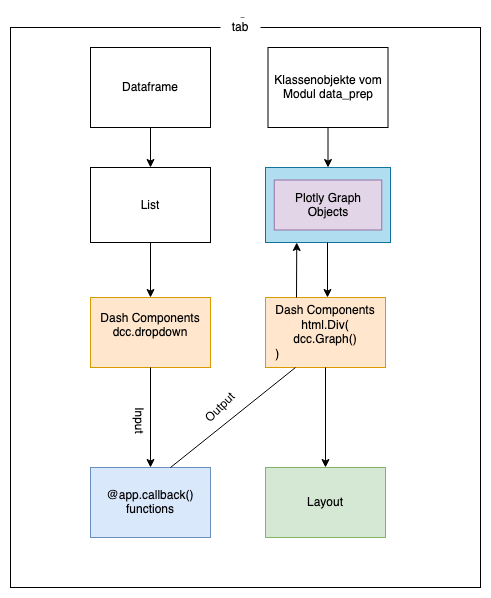
\includegraphics[width=8cm, height=10cm]{ablauf_dash_mit_cb}
    %         \caption{Ablauf Tab mit Callback}
    %         \label{fig:process tab_dash_cb}
    % \end{figure}
 
    Der Callback übergibt den Wert (input\_value) des Dropdown-Menüs an die Funktion \texttt{update\_output\_div()}. 
    Die Funktion gibt das Ergebnis einer \texttt{fig\_()}-Funktion mit diesem Wert als Argument zurück.\footnote{Diese Funktionen übergeben den Methoden der Kindklassen aus dem Modul \texttt{data\_prep} das Argument. 
    Diese erzeugen einen Dataframe basierend auf den übergebenden Argument und geben mit Hilfe der Plotly-Funktionen ein Plotly Graph Object Figure der gefilterten Daten zurück.}
    Der Callback \texttt{@app.callback} übergibt das zurückgegebene Ergebnis an die im Output angegebene Komponente.
    
    Input() und Output() nehmen die id einer Komponente und die Eigenschaft einer Komponente als Argumente entgegen.
    Die Inputkomponente ist in dem Beispiel die Dropdown-Komponente, während die Outputkomponente die dcc.Graph-Komponente der
    \texttt{html\_\_use\_by\_month()} darstellt. Beide werden über die eindeutige \texttt{component\_id} adressiert.
    Multiple Inputs and Outputs sind ebenfalls möglich. So sind in der \texttt{expenditures\_app.py}
    jeweils zwei Diagramme und Zahlenwerte für den Umsatz von den Werten einer Dropdown-Liste abhängig.
    % Dabei handelt es sich um Methoden, die die Daten nach einem Wert filtern und die vom Wert der Dropdown-Liste abhängig sind. Deswegen wird bei diesen
    % Plotly-Funktionen in der Tab-Datei der Wert der Dropdown-Liste als Argument mit in die Funktion gegeben.
    In der folgenden Abbildung ist die Ablauflogik in den Tab-Dateien mit der Callback-Funktion zu sehen.

    \begin{figure}[H]
        \centering
            \includegraphics[width=12cm, height=10cm]{ablauf_tab_cb_ps}
            \caption{Ablauf Tab mit Callback}
            \label{fig:process tab_dash_cb}
    \end{figure}


    Zusammengesetzt wird das Layout des Dashboards durch den Aufruf der Layout-Funktion der einzelnen Tab-Dateien in der \texttt{index.py}.
    Die \texttt{index.py} definiert zudem das Layout des gesamten Dashboards. Hier werden auch die Anzahl und die Eigenschaften der Tabs festgelegt. 
    Die Dekorator-Callback-Funktion \texttt{@app.callback()} steuert die Auswahl der Tabs und ruft die jeweiligen Tabs beziehungsweise deren 
    Layouts auf. \autoref{fig:process tab_dash_cb} zeigt im Allgemeinen die Funktionsweise einer Tab-Datei mit der \texttt{index.py}.

    \begin{figure}[H]
        \centering
            \includegraphics[width=15cm, height=10cm]{ablauf_tab_cb_ind_ps}
            \caption{Ablauf Tab mit index}
            \label{fig:process tab_dash_cb}
    \end{figure}

    Der Einstiegspunkt zur Ausführung des Dashboards ist die Datei \texttt{index.py}. Mit dieser Datei wird das Dashboard mittels \texttt{Flask-Webserver}
    gestartet. Zur Vermeidung zirkulärer Importe ist die Dash-Instanz in der separaten \texttt{app.py} definiert\cite[vgl.][]{plotly_url_2021}.


    %\textit{Standardbericht}\\

\section{Demonstration der Funktionalität}

    Im Folgenden wird die Funktionsweise des Systems dargelegt. Dabei wird zunächst auf Voraussetzungen eingegangen und dann
    spezifisch auf das Teilsystem 1 Import und schließlich der
    praktische Import der Daten skizziert. Da das Teilsystem 2 keine Schnittstelle
    nach außen bietet, wird auf dieses nicht eingegangen. Teilsystem 3 ist von Interesse, da von diesem das Dashboard
    gestartet wird. Das Dashboard ist die grafische Umsetzung des Teilsystem 2 und Teilsystem 3. Beim Dashboard wird noch kurz auf das Layout
    eingegangen, bevor die Funktionsweise und die Datenvisualisierungen besprochen werden.


    \subsection{Technische Voraussetzungen}
    Der Programmcode zum Projekt ist auf github zu finden.\footnote{\url{http://pfad/zu/github/repo}} Dort gibt es weitere Informationen zur Installation.
    Das System wurde auf den Betriebssystemen macOS Big Sur, Linux in der Ubuntu-Distribution 20.10. getestet.
    Das Dashboard kann mit auf den aktuellen Versionen der Web-Browser Google Chrome, Firefox und Safari dargestellt werden. 
    Als Hardware-Anforderungen wird ein Intel Dual Core i5 (Haswell) mit 128 GB Festplatte und 8 GB Arbeitsspeicher angegeben. 
    Mit dem Programmcode werden keine bibliothekarischen Daten mitgeliefert.\footnote{Testdaten werden nach der Veröffentlichung des Repositoriums voraussichtlich
    bereitgestellt.}
    
    \subsection{Daten-Import}
    Der Import der Daten findet über Skripte statt. Diese liegen im Projektverzeichnis \texttt{src/instances}.
    Für Budget, Umsatz, Neuerwerbungen und Ausleihdaten liegen einzelne Python-Skripte bereit, die manuell über die Kommandozeile
    aufgerufen werden können. Zudem gibt es noch ein shell-Skript, das die vier Skripte zusammen anstösst. Dieses
    muss ebenfalls manuell aufgerufen werden.
    Nach erfolgreichem Import der Dateien aus den Importverzeichnissen wird eine einfache Erfolgsmeldung auf der Kommandozeile ausgegeben.
    %\footnote{Es gibt Warnungen, die angezeigt werden. Diese Warnmeldungen haben keinen Einfluss auf den Import. Im Bearbeitungszeitraum der Arbeit konnte diesen Warnmeldungen leider nicht nachgegangen werden.}

    Die Pfade zu den lokalen Verzeichnissen für Import und Speicherung der Daten sind als Konstanten zentral in der configuration.py 
    im Projektverzeichnis hinterlegt. Dort sind auch noch andere Pfadkonstanten definiert, die auf Dateien für die Datenanreicherung verweisen, welche das Teilsystem 1
    und das Teilsystem 2 unterstützen. Wichtig ist, dass die zu importierenden Daten über Dateinamen einer gewissen Semantik und 
    über ein gewisses Format verfügen, sonst werden sie nicht importiert (Siehe auch \autoref{chap:five_one_three} Teilsystem 1).

    \subsection{Dashboard}
    Gestartet wird die Dashboard-Application auf der Kommandozeile, indem \texttt{index.py} im Projektverzeichnis \texttt{dashboard}
    aufgerufen wird. Diese startet den Flask-Webserver mit der Dashboard-App. Der Webserver ist in der \texttt{index.py} so eingestellt, 
    dass er an allen Netzwerkschnittstellen lauscht.


    \begin{figure}[H]
        \centering
            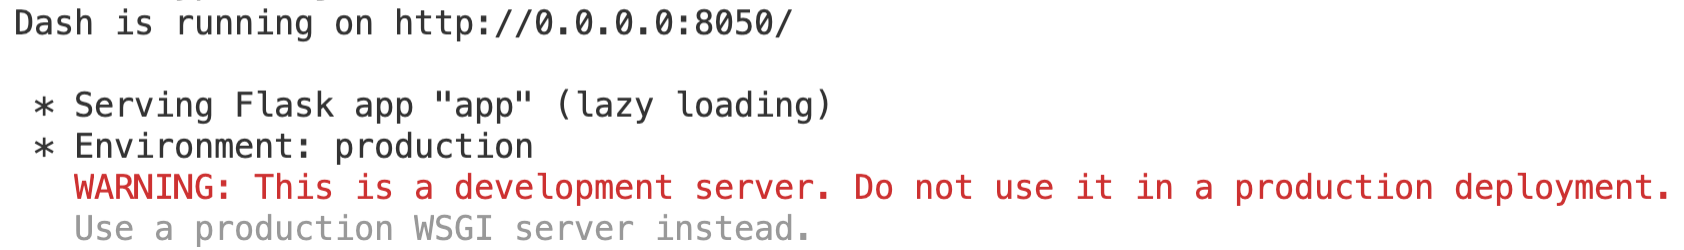
\includegraphics[width=12cm, height=2cm]{flask_webserver}
            \caption{Start Flask Webserver}
            \label{fig:flask}
    \end{figure}

    % Wie im \autoref{chap:five_one_three} Teilsystem 3 beschrieben besteht das Dashboard aus drei Tabs.
    % Die Navigation zu den drei Tabs ist im oberen Bereich des Dashboards nebeneinander angeordnet. 
    
    % \begin{figure}[H]
    %     \centering
    %         
\includegraphics[width=14cm, height=2cm]{tabs}
    %         \caption{Tabs-Navigation}
    %         \label{fig:flask}
    % \end{figure}
    Das Dashboard kann mit der angegebenen Adresse vom Web-Browser geöffnet werden.
    \autoref{fig:Struktur Layout} zeigt schematisch die Layout-Struktur des Dashboards. 


    \begin{figure}[H]
        \centering
            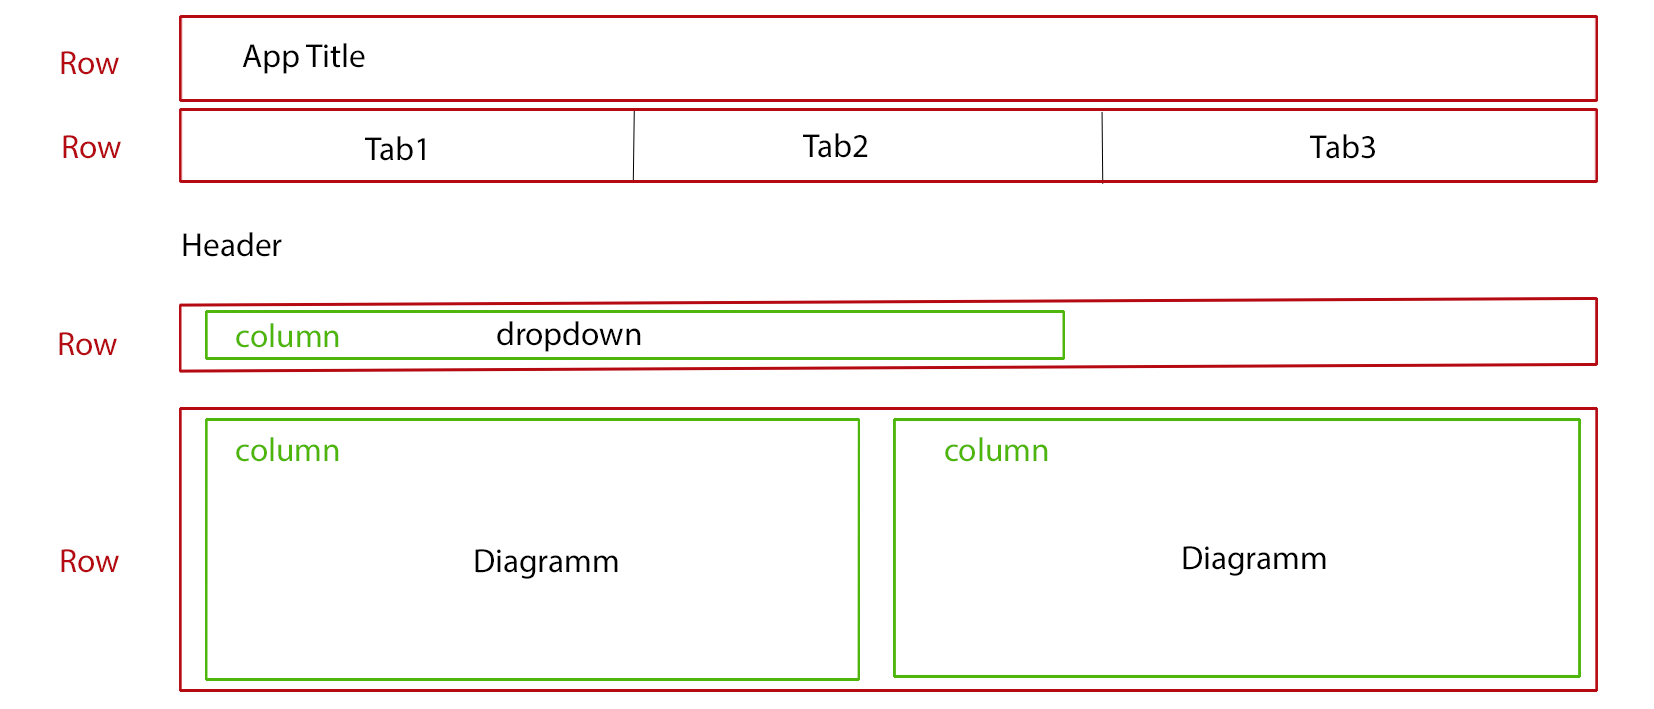
\includegraphics[width=14cm, height=6cm]{layout_abstr}
            \caption{Struktur Layout}
            \label{fig:Struktur Layout}
    \end{figure}


    Die Layout-Struktur besteht aus Divs, Rows, Header und Columns, und den Steuerelementen wie Dropdown-Menüs sowie den Darstellungselementen wie Diagrammen oder
    Cards. Die einzelnen Rows werden durch Div-Container bemantelt. Diese sind auf dem html-Body angesiedelt.
    Während die ersten beiden Reihen zentral in der \texttt{index.py} festgelegt werden, werden die anderen Reihen in den einzelnen Tab-Dateien definiert. 
    Diese beherbergen bis zu drei Columns-Elemente, in denen die Steuer- und Datenvisualisierungselemente enthalten sind.
    Die Columns-Elemente sind in Abhängigkeit der darzustellenden Daten unterschiedlich groß. 
    Die Größe wird festgelegt in den einzelnen \texttt{fig\_()}-Funktionen des Teilsystems 3.
    Die Header gelten als inhaltlicher Trenner zwischen den einzelnen Datenvisualisierungen und dienen der schnelleren Orientierung. 
    Die Header sind mit der jeweils nachfolgenden Row verknüpft. Das Dashboard besteht aus drei Tabs: \textit{Umsatz und Budget}, 
    \textit{Lesesaal und Ausleihe}, \textit{Neuerwerbungen und Bestand}. Der Wechsel zwischen den Tabs geschieht durch das einmalige
    Klicken mit der Maus auf dem Tab-Titel. Nachdem die Adresse im Browser geöffnet wurde, wird der Tab \textit{Umsatz und Budget} aufgerufen. Dieser ist
    als default-value im Dashboard-Layout der \texttt{index.py} eingestellt.

    \clearpage
    \noindent
    \textit{Tab1 - Umsatz und Budget}\\ 
    Den Tab \textit{Umsatz und Budget} zeigt \autoref{fig:tab1}.\footnote{Für die Darstellung der Umsatz- und
    Budgetdaten werden sowohl die Kostenstellen als auch die Lieferanten maskiert dargestellt. Es wurde außerdem mit Testdaten
    gearbeitet, die bis März 2021 gehen.}

    % \KOMAoptions{paper=A3,paper=portrait}
    % \recalctypearea

    \begin{figure}[H]
        \centering
            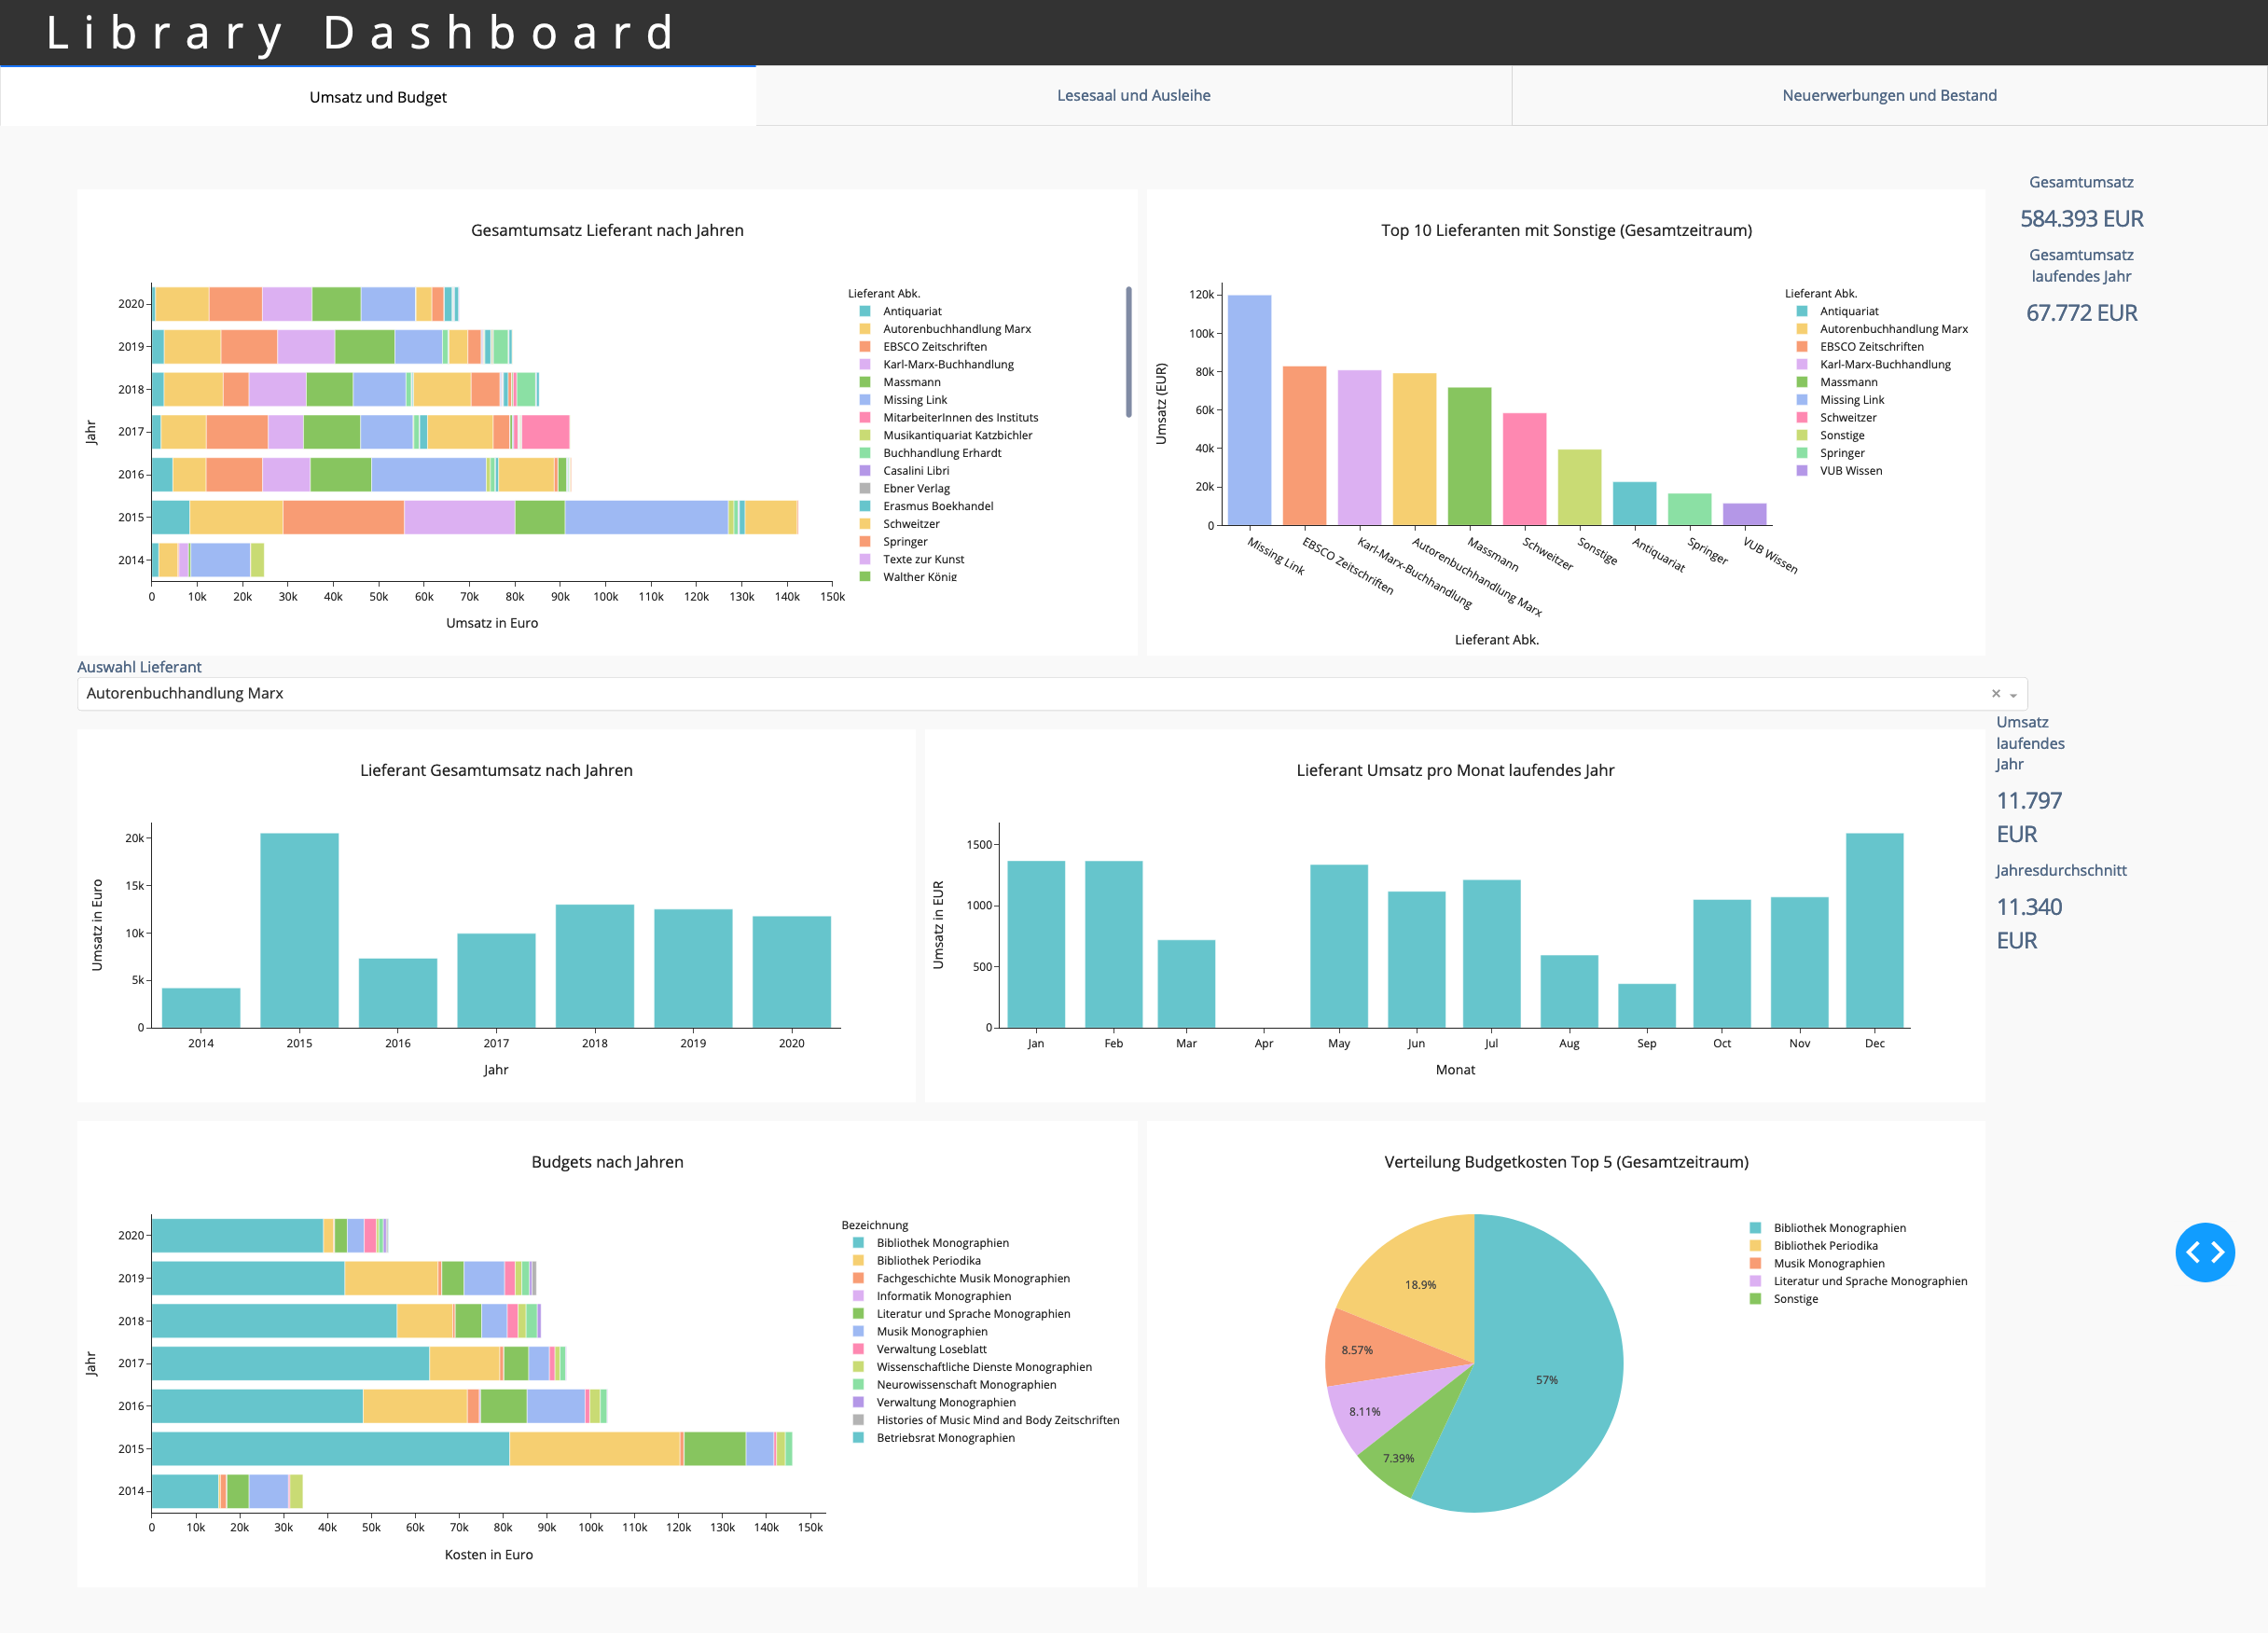
\includegraphics[width=16cm, height=17.0cm]{tab1}
            \caption{Tab1}
            \label{fig:tab1}
    \end{figure}


    % Genug A3 fürs erste. Jetzt ein Seitenumbruch und dann wieder A4-Format:
    \clearpage
    % \KOMAoptions{paper=A4,paper=portrait}
    % \recalctypearea
    
    Folgende Diagramme und Steuerelemente werden im Tab \textit{Umsatz und Budget}.
    \begingroup
    \setlength{\tabcolsep}{12pt} % Default value: 6pt
    %\renewcommand{\arraystretch}{1.0}
    \begin{table}[h]
        \LARGE
        \centering
        \begin{adjustbox}{max width=\textwidth}
        \begin{tabular}{p{0.1\textwidth}p{0.5\textwidth}p{0.4\textwidth}p{0.25\textwidth}p{0.4\textwidth}p{0.5\textwidth}}
           \toprule
           Row        &Titel &Beschreibung &Datenset &Darstellung &Interaktivität auf dem Dashboard\\
           \midrule
            1           &Gesamtumsatz Lieferant nach Jahren &Die Einzelwerte der Lieferanten pro Jahr werden dargestellt.   &Umsatzdaten    &gestapeltes Balkendiagramm (horizontal)    &Plotly-Interaktivität (Aus- und Einblenden von Balken, Hover-Informationen)\\
                        &Top 10 Lieferanten mit Sonstige (Gesamtzeitraum)   &Die 9 Lieferanten, bei denen der Umsatz am stärksten ist, werden dargestellt. Die restlichen werden in der Kategorie Sonstiges gruppiert.   &Umsatzdaten    &Balkendiagramm    &Plotly-Interaktivität (Aus- und Einblenden von Balken, Hover-Informationen)\\
                        &Gesamtumsatz&-&Umsatzdaten    &nummerischer Wert   &-\\
                        &Gesamtumsatz laufendes Jahr&-&Umsatzdaten    &nummerischer Wert   &-\\
            
                        \midrule
            2           &Auswahl  Lieferant &Dropdown-Menü mit eindeutigen Werten der Dataframe-Spalte \enquote{Lieferanten Abk.}&Umsatzdaten&Dropdown-Menü &Auswahl von Werten aus einer Liste. Dadurch werden vier Darstellungen beeinflusst.\\
            \midrule
            3           &Lieferant Gesamtumsatz nach Jahren&Der Gesamtumsatz eines Lieferanten nach Jahren wird dargestellt.   &Umsatzdaten    &Balkendiagramm    &Auswahl des Lieferanten über das Dropdown-Menü\\
                        &Lieferant Umsatz pro Monat laufendes Jahr&Der Gesamtumsatz eines Lieferanten nach Monaten für das laufende Jahr wird dargestellt.   &Umsatzdaten    &Balkendiagramm    &Auswahl des Lieferanten über das Dropdown-Menü\\
                        &Umsatz laufendes Jahr (für einen Lieferanten)&- &Umsatzdaten    &numerischer Wert    &Wert verändert sich durch Auswahl des Lieferanten über das Dropdown-Menü\\
                        &Jahresdurchschnitt (Lieferant)&- &Umsatzdaten    &numerischer Wert    &Wert verändert sich durch Auswahl des Lieferanten über das Dropdown-Menü\\
            \midrule
            4           &Gesamtbudget Kostenstellen nach Jahren&Die Einzelwerte der Kostenstellen pro Jahr werden dargestellt.&Budgetdaten    &gestapeltes Balkendiagramm (horizontal)    &Plotly-Interaktivität (Aus- und Einblenden von Balken, Hover-Informationen)\\
                        &Budgetkosten Top 5 Kostenstellen mit Sonstige (Gesamtzeitraum)&Die 4 Kostenstellen, bei den die Budgetkosten am größten sind, werden dargestellt. Die restlichen werden in der Kategorie Sonstiges gruppiert. &Budgetdaten    &Kreisdiagramm    &Plotly-Interaktivität (Aus- und Einblenden von Anteilen, Hover-Informationen)\\

        \bottomrule
        \end{tabular}
        \end{adjustbox}
        \caption
        \end{table}
    \endgroup
    


\clearpage
\noindent
\textit{Tab2 - Lesesaal und Ausleihe}

Den Tab \textit{Lesesaal und Ausleihe} zeigt \autoref{fig:tab2}.

    \begin{figure}[H]
        \centering
            \includegraphics[width=16cm, height=18cm]{tab2_1}
            \caption{Tab2}
            \label{fig:tab2}
    \end{figure}
    
\clearpage
Folgende Diagramme, Tabellen und Steuerelemente werden im Tab \textit{Lesesaal und Ausleihe} dargestellt.


    \begingroup
    \setlength{\tabcolsep}{12pt} % Default value: 6pt
    %\renewcommand{\arraystretch}{1.5} 
    \begin{table}[h]
        \LARGE
        \centering
        \begin{adjustbox}{max width=\textwidth}
        \begin{tabular}{p{0.1\textwidth}p{0.5\textwidth}p{0.4\textwidth}p{0.3\textwidth}p{0.4\textwidth}p{0.4\textwidth}}
           \toprule
           Row        &Titel &Beschreibung &Datenset &Darstellung &Interaktivität auf dem Dashboard\\
           \midrule
            1           &Auswahl  Jahr &Dropdown-Menü mit eindeutigen Werten der Dataframe-Spalte \enquote{Jahr}.&Ausleihdaten&Dropdown-Menü &Auswahl von Werten aus einer Liste. Dadurch werden eine Darstellung beeinflusst.\\
           \midrule
            2           &Monatliche Anzahl der Nutzer:innen nach Servicezeit-Gruppen&Es wird der monatliche Verlauf nach den vier Service-Zeiten dargestellt.&Lesesaaldaten&Liniendiagramm&Auswahl des Zeitraums (Jahr) über Dropdown-Menü. Plotly-Interaktivität (Aus- und Einblenden von Linien, Hover-Informationen)\\
                        &Jährliche Lesesaalnutzung nach Servicezeit-Gruppen&Es wird die jährliche Nutzung des Lesesaal in den Service-Zeiten dargestellt.&Lesesaaldaten&Balkendiagramm    &Plotly-Interaktivität (Aus- und Einblenden von Balken, Hover-Informationen)\\          
            \midrule
            3           &Jährliche Ausleihe nach den Top 10 RVK-Fachsystematiken mit Sonstige&Die 9 Fachsystematiken, bei denen die Ausleihanzahl am größten ist werden dargestellt. Die übrigen Fachsystematiken im Bestand werden in der Kategorie Sonstiges gruppiert.&Ausleihdaten&gestapeltes Balkendiagramm (horizontal)&Plotly-Interaktivität (Aus- und Einblenden von Balken, Hover-Informationen)\\
                        &Gesamtverteilung Ausleihe Buchservice / Bibliothek&Es wird die prozentale Verteilung zweier Werte dargestellt.&Ausleihdaten    &Kreisdiagramm   &Plotly-Interaktivität (Aus- und Einblenden von Anteilen, Hover-Informationen)\\
            \midrule
            4           &Tabellarische Darstellung der 5 besonders nachgefragten Titel nach Jahren&-&Ausleihdaten    &Tabelle mit den Spalten Jahr, Signatur, Titel und Anzahl der Ausleihen.&-\\

        \bottomrule
        \end{tabular}
        \end{adjustbox}
        \caption
        \end{table}
    \endgroup



    \clearpage
    \noindent
    \textit{Tab3 - Neuerwerbungen und Bestand}
    
    Den Tab \textit{Neuerwerbungen und Bestand} zeigt \autoref{fig:tab3}.

    
    \begin{figure}[H]
        \centering
            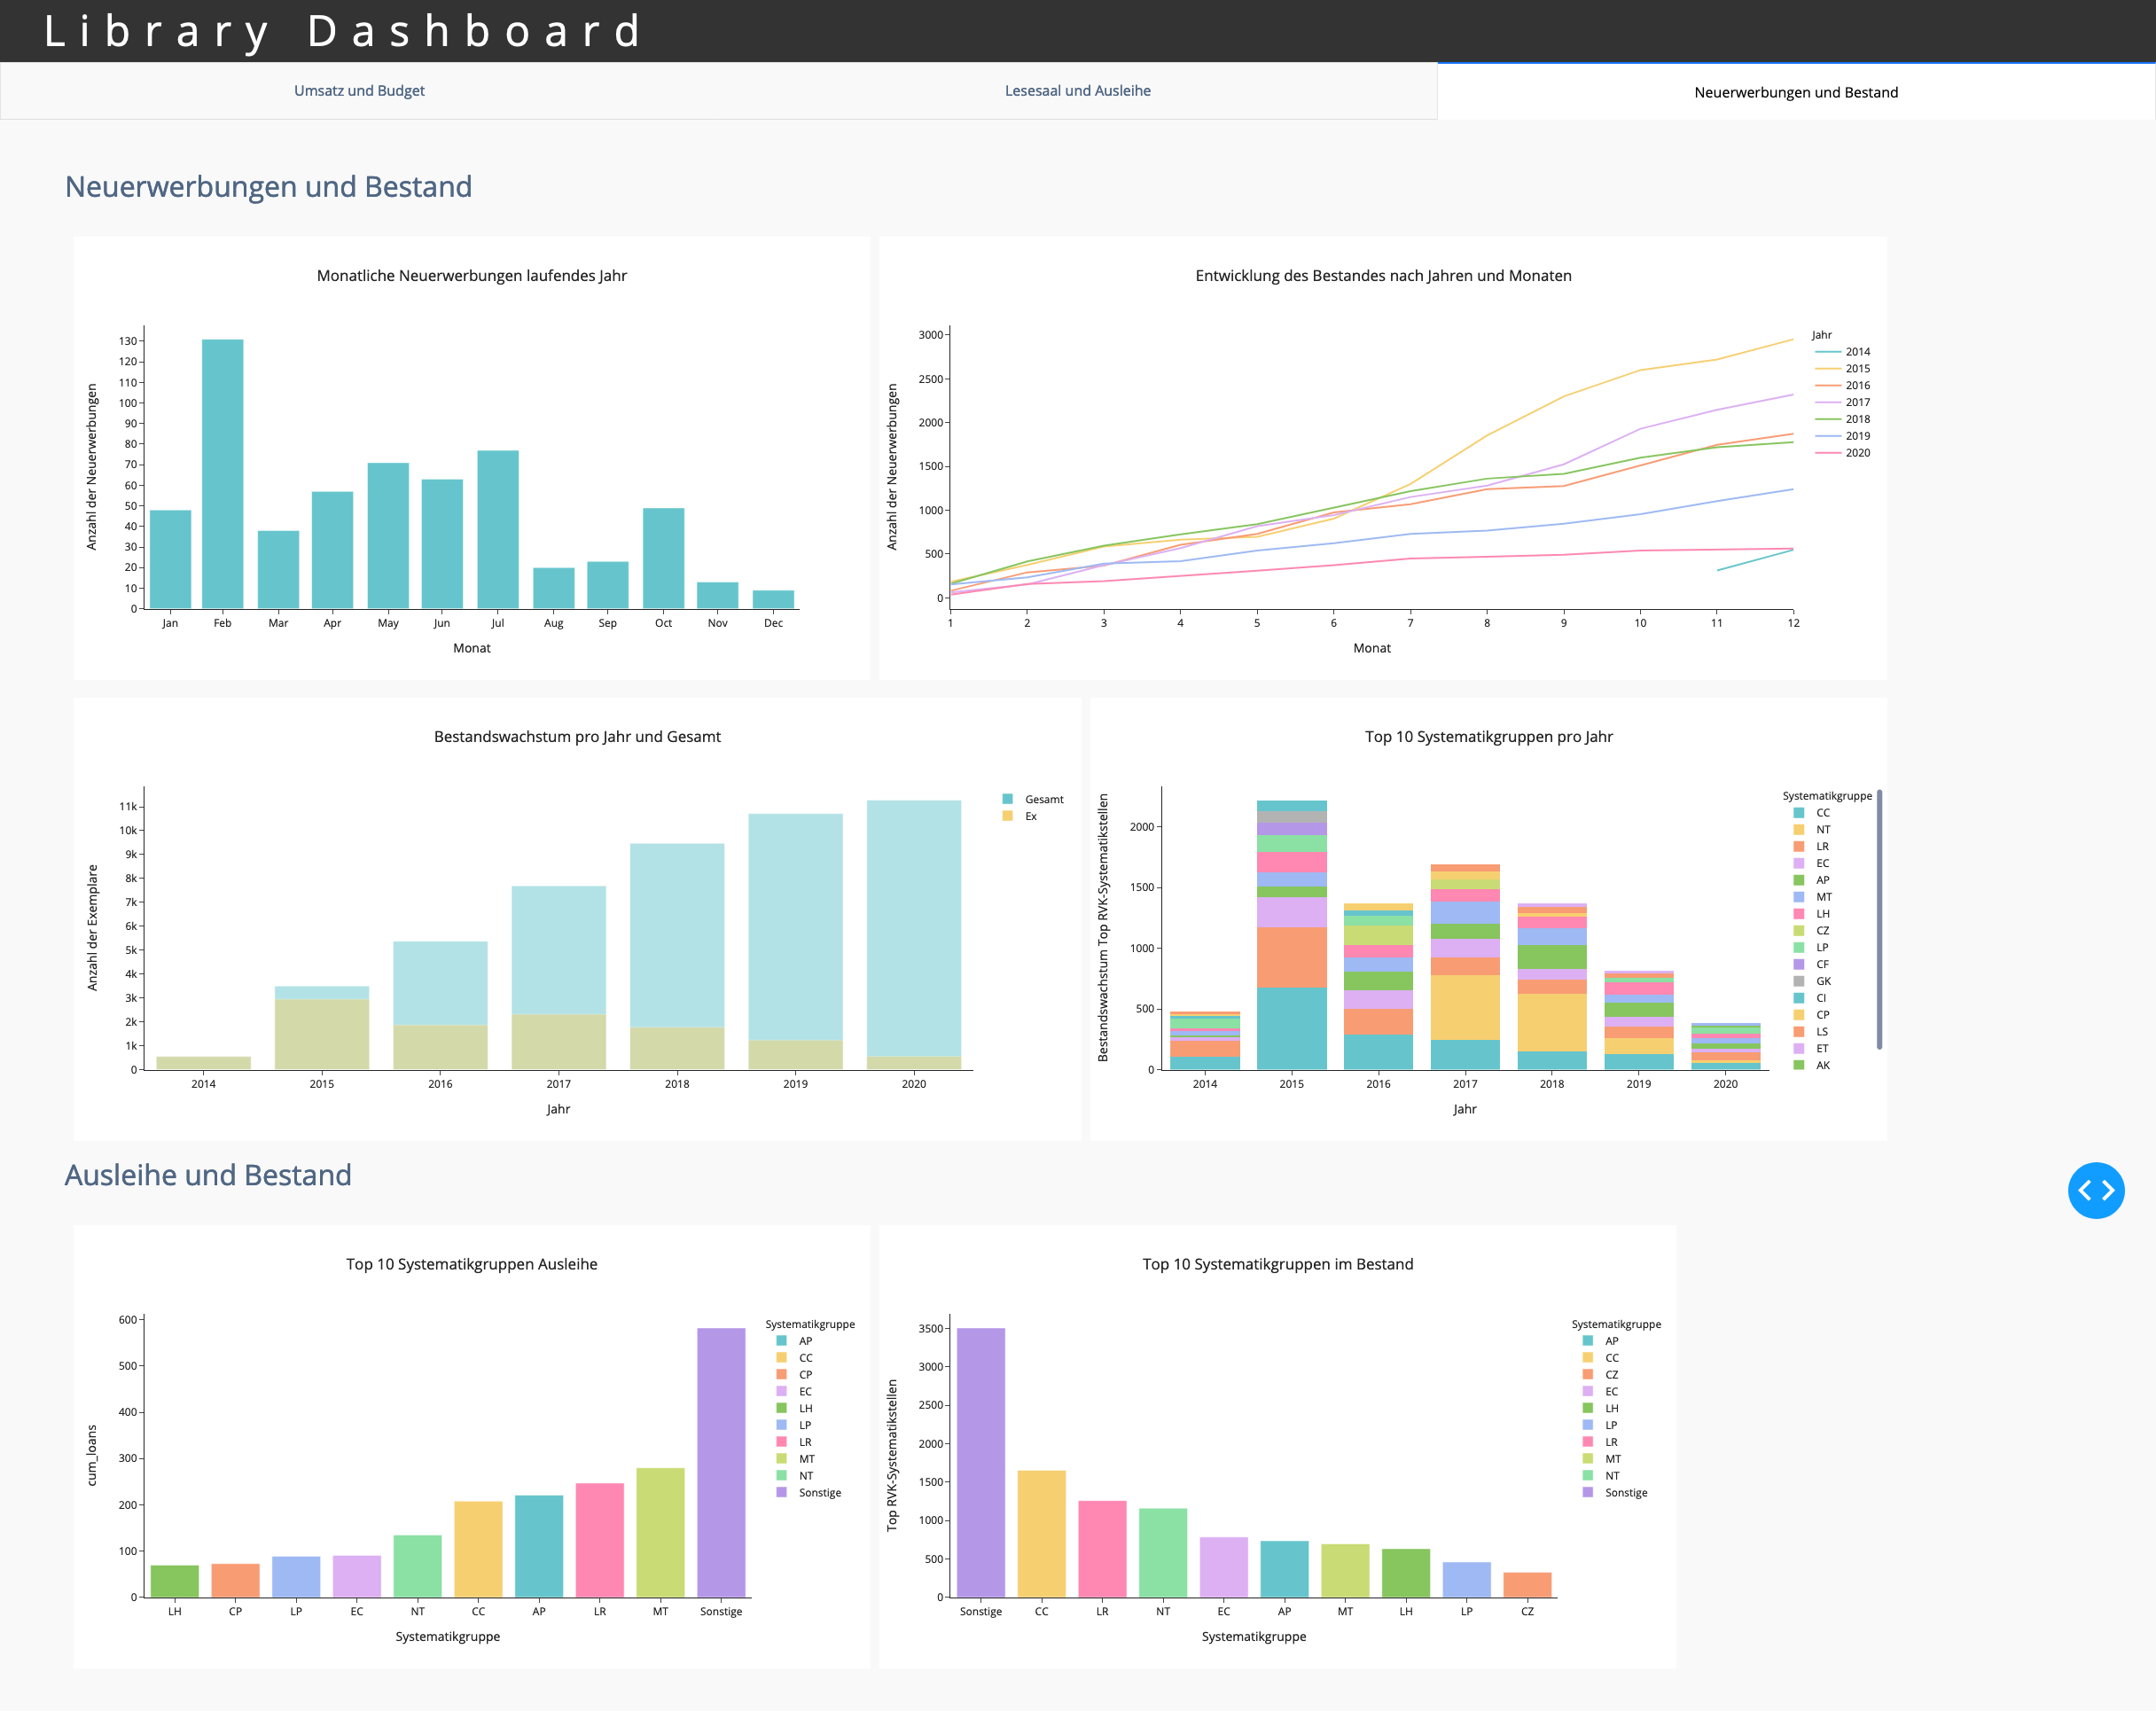
\includegraphics[width=16cm, height=18cm]{tab3}
            \caption{Tab3}
            \label{fig:tab3}
    \end{figure}

    \clearpage
    Folgende Diagramme werden im Tab \textit{Neuerwerbungen und Bestand} dargestellt.
    

    \begingroup
    \setlength{\tabcolsep}{12pt} % Default value: 6pt
    %\renewcommand{\arraystretch}{1.5} 
    \begin{table}[h]
        \LARGE
        \centering
        \begin{adjustbox}{max width=\textwidth}
        \begin{tabular}{p{0.1\textwidth}p{0.5\textwidth}p{0.4\textwidth}p{0.3\textwidth}p{0.4\textwidth}p{0.4\textwidth}}
           \toprule
           Row        &Titel &Beschreibung &Datenset &Darstellung &Interaktivität auf dem Dashboard\\
           \midrule
            1           &Monatliche Neuerwerbungen laufendes Jahr&Es werden die monatlichen Neuwerwerbungen des laufenden Jahres dargestellt.&Bestandsdaten&Balkendiagramm&-\\
                        &Jährliche Bestandsentwicklung nach Monaten&Darstellung des akkumulierten Bestandswachstums für die einzelnen Jahre&Bestandsdaten&Liniendiagramm    &Plotly-Interaktivität (Aus- und Einblenden von Linien, Hover-Informationen)\\          
            \midrule
            2           &Bestandswachstum pro Jahr und Gesamt&Darstellung des absoluten und des relativen Wachstums nach Jahren.&Bestandsdaten&überlagertes Balkendiagramm&Plotly-Interaktivität (Aus- und Einblenden von Balken, Hover-Informationen)\\
                        &Top 10 Systematikgruppen pro Jahr&Die jährlichen Top 10 Fachsystematikgruppen im Bestand werden dargestellt.&Bestandsdaten    &gestapeltes Balkendiagramm&Plotly-Interaktivität (Aus- und Einblenden von Balken, Hover-Informationen)\\
            \midrule
            3           &Top 10 Systematikgruppen Ausleihen&Es werden die Top 10 Fachsystematiken der Ausleihe vom kleinsten Wert zum größten des Bestandes (ohne Buchservice) dargestellt.&Ausleihdaten&Balkendiagramm&Plotly-Interaktivität (Aus- und Einblenden von Balken, Hover-Informationen)\\
                        &Top 10 Systematikgruppen Bestand&Es werden die Top 10 Fachsystematiken im Bestand vom größten Wert zum kleinsten dargestellt.&Bestandsdaten&Balkendiagramm&Plotly-Interaktivität (Aus- und Einblenden von Balken, Hover-Informationen)\\

        \bottomrule
        \end{tabular}
        \end{adjustbox}
        \caption
        \end{table}
    \endgroup

\section{Bewertung}

\subsection{Allgemeines}
\label{chap:five_three_one}
Das Ziel des vorliegenden Projektes war es, ein Proof-of-Concept eines Systems zu entwickeln, 
das wesentliche bibliothekarische Daten sammelt, statistisch mit geeigneten Methoden und
Datenvisualisierungen analysiert und auswertet. Als Ergebnis steht ein datengetriebenes 
Unterstützungssystem, das durch drei Teilsysteme den Import und eine erste Bereinigung der Daten,
die Aufbereitung der Daten, die Umwandlung der Daten in Datenvisualisierungen und deren Darstellung garantiert. 
Das System verarbeitet die bibliothekarischen Daten aus den Bereichen Umsatz und Budget, Lesesaal und Ausleihe 
sowie der Bestandsentwicklung.

Das System ist ausgelegt auf diese strukturierten Daten, die aus heterogenen Datenquellen stammen.
Diese Daten bringen Anforderungen wie Datenbeschaffenheit oder Dateiformatspezifikationen mit, 
die den Prozess der Datenintegration in das System bestimmen. Es konnte mit dem System gezeigt werden, 
dass diese Anforderungen für die vorliegenden Daten vom System erfüllt wurden, indem die Prozesse 
der drei Teilsysteme für diese Daten entwickelt wurden. 

So erwartet das System beim Import die Daten in einer gewissen Struktur (Datenformat). 
Überdies muss das Dateiformat dem System bekannt sein und der Dateiname speziellen semantischen 
Kriterien entsprechen. Wenn diese Anforderungen erfüllt sind, können die Daten problemlos in das System integriert werden.
Weiterhin können bestimmte Modifikation im Teilsystem 1 eingestellt werden wie die Entfernung
bestimmter Zeichen. Diese Modifikation sind aber sehr einfach und wurden aus der Voranalyse
der Daten entwickelt. Die Modifikationen können zwar auf andere Daten angewendet werden, gelten aber ersteinmal nur für die vorliegenden Daten. 
Darüberhinaus bietet das System keine weiteren einstellbaren Möglichkeiten an. Ferner ist das System auf einfache 
Tabellenstrukturen, wie sie in tsv- oder Excel-Dateien abgespeichert werden können, ausgerichtet.
Grundsätzlich erfolgt der Import der Daten (einfache Tabellenstrukturen) aus heterogenen Datenquellen 
in einfache Tabellenstrukturen in einem einheitlichen csv-Dateiformat. Der einfache Import von Daten von einem Dateiformat 
in das csv-Format ist problemlos möglich, wenn Daten vorliegen, die keine weiteren speziellen
Anforderungen besitzen.

Das Teilsystem 2 und das Teilsystem 3 erwarten csv-Dateien, die sie weiterverarbeiten können. 
Deshalb kann das System auch unabhängig vom Teilsystem 1 funktionieren. 
Vielmehr stellt das Teilsystem 1 eine Möglichkeit dar, wie der Import der Daten ablaufen kann. 
Das Teilsystem 1 wurde für das System entwickelt, da insbesondere mit den vorliegenden Daten umgegangen werden musste und ebenfalls hier 
der Großteil der Datenanreicherung abläuft.


\subsection{Datenlage im vorliegenden System}
In dem vorliegenden Projekt wurden hauptsächlich die heterogenen Bibliotheksdaten aus dem \textit{\acrshort{hebis}}-Verbund sowie aus dem \textit{\acrlong{LBS}} Frankfurt verarbeitet.
Da potentiell alle Bibliotheken, die durch das \textit{\acrshort{LBS}}-Team Frankfurt betreut werden, die gleichen Daten zur Verfügung gestellt bekommen,
kann das vorliegende  System von diesen Bibliotheken implementiert werden. Eine Aussage darüber, ob es in anderen Bibliotheken oder Verbünden implementiert werden kann, die ebenfalls
Instanzen des \textit{\acrlong{CBS}s} und \textit{\acrshort{LBS}} betreiben, kann leider hier nicht getroffen werden, da die technische Infrastruktur
und die Datenbereitstellung stark differieren können. 

Der Workflow für den Import, die Weiterverarbeitung und die Darstellung der Umsatz- und Budgetdaten sowie der Bestandsdaten kann durch das System
abgedeckt werden, da die hierfür benötigten Daten der Bibliothek regelmäßig zur Verfügung gestellt werden. Die Ausleihdaten werden nicht automatisch
geliefert. Dadurch entsteht eine Schieflage zwischen Bestands- und Ausleihdaten in Bezug auf die Bestandsgröße.
Deshalb müssten im Regelbetrieb die bibliotheksinternen Prozesse und das System angepasst werden, um einen regelmäßigen Abzug der Ausleihdaten
verarbeiten zu können. Zur Zeit ist das System auf die vorliegenden Daten zugeschnitten.

% Data is messy - Library data too!
Teilweise mussten die Daten aufgrund von Unzulänglichkeiten angepasst und bearbeitet werden.
Zu nennen wären hier fehlende Daten in den Umsatz- und Budgetdaten. Diese fehlenden Daten können Fehler in der Darstellung im Dashboard erzeugen.\footnote{Ebenso fehlen noch relevante Lieferanten, die sich nicht im \textit{\acrshort{LBS}} finden lassen.}
Des Weiteren wird bei dem monatlichen Abzug der Neuerwerbungsdaten aus dem \textit{\acrshort{CBS}} Duplikate mit exportiert. Diese Duplikate entstehen durch
die Mehrfachexemplare, die an einem Datensatz hängen. Diese lassen sich zwar als Duplikate relativ einfach über die Signatur erkennen und entfernen.
Darunter würden dann aber auch alle ebooks fallen, da sie die gleiche Signatur aufweisen.

Mit diesen Ausnahmen innerhalb der Daten musste und wurde ein Umgang gefunden. Diese haben mitunter alle Teilsysteme affektiert und
die Programmierung dieser mitbestimmt.

In Bezug auf die Darstellung der Daten im Dashboard stellt die Vielzahl von diskreten Werten ein Problem dar. 
Die Grenze der Darstellbarkeit der Daten in Form von Diagrammen ist erreicht, wenn zu viele diskrete Werte dargestellt werden müssen.
Das betrifft zum Beispiel die Vielzahl an Lieferanten in dem Diagramm \enquote{Gesamtumsatz Lieferant nach Jahren} im Tab \textit{Umsatz und Budget}. 
Dort kann anhand der Farbe in den gestapelten Balkendiagramm nicht mehr zwischen den einzelnen Lieferanten unterschieden werden, da die Color-Palette 
nur eine bestimmte Anzahl an diskreten Werten darstellen kann \cite[Vgl.][]{plotly_discrete_2021}.\footnote{Auch wäre die Frage zu stellen, inwieweit hier die Darstellung aller Lieferanten sinnvoll im Hinblick auf die Informationsrezeption.}
Ebenso betrifft dieses Problem die Auswertung der Daten nach den \textit{\acrshort{RVK}}-Fachsystematiken beziehungsweise nach deren Untergruppen. 
Erste Datenanalysen haben verdeutlicht, dass es eine nicht darstellbare Anzahl an Fachsystematiken im Bestand der Bibliothek gibt, durch die eine visuelle Darstellung nicht zielführend ist.
Aufgrund dieser Darstellungsprobleme wurden zusätzlich noch andere Diagramme erstellt, die die Anzahl der darzustellenden Werte durch bestimmte Clusterungen reduziert.
So wurde ein Diagramm erstellt, das eine bestimmte Anzahl der umsatzstärksten Lieferanten im Gesamtzeitraum zeigt. Bei den \textit{\acrshort{RVK}}-Fachsystematiken wurde ebenso
verfahren.




% Die Konzeption des Prototyps ist immer auch rückwertsgewand.
% Das Proof-of-Concept ist ausgelegt auf bestimmte Daten wie Umsatz- und Budgetdaten, Ausleih- und Bestandsdaten sowie Lesesaaldaten 
% aus dem bibliothekarischen Bereich. Diese strukturierten Daten stammen aus heterogenen Datenquellen und bringen bestimmte 
% Anforderungen wie Datenbeschaffenheit oder Dateiformatspezifikationen mit, die den Prozess der Integration bestimmen.
% Diese Anforderungen wurden durch das vorliegende System erfüllt, indem es auf diese Daten zugeschnitten wurde.


% Während das System verschiedene Dateiformate beim Import der Rohdaten unterstützt und um neue relativ leicht erweitert werden kann, 
% ist das System nicht dazu ausgelegt bei Veränderungen der inhaltlichen Struktur der Datenformate flexibel reagieren zu können. 
% Das System verhält sich mitunter blind gegenüber den Datenformaten und erwartet sie einer spezifischen Form. 
% Es gibt aber basale Möglichkeiten im Teilsystem 1 durch die Parametersetzung im Programmcode steuernd einzugreifen. 
% Der Aufwand inwiefern dass System bei einer inhaltlichen Änderung der Datenformate geändert werden müsste, 
% hängt natürlich auch vom Grad der Datenformatsänderung ab. Ändert sich zum Beispiel die Spaltenanzahl einer Tabelle in den zu importierenden Daten, 
% hat dieses auch Auswirkungen auf die bereits importierten Daten. Eine Konsequenz wäre hier, dass nach erfolgreichem Export die Änderung die Datei mit den 
% ‚Altdaten‘ für die weitere Auswertung durch das Teilsystem 2 bricht. Diese Veränderung würde vermutlich eine tiefgreifende Veränderung des Systems nachsichziehen 
% und einen hohen zeitlichen Aufwand für Problembehebung bedeuten. Ebenso problematisch wäre es, wenn sich zum Beispiel die Werte in den Spalten ändern würden. Andererseits können auch Daten, die schon im Csv-Format vorliegen direkt vom Teilsystem 2 bearbeitet werden, 
% da das Teilsystem 1 unabhängig von den anderen Teilsystemen arbeitet.


% Die Integration neuer Datenquellen ist mit dem System prinzipiell möglich. 
% Wie hoch hier der Aufwand ist, hängt wiederum sehr von den neuen Datenquellen ab. 
% Je heterogener die Datenquellen sind und je heterogener die Daten selber beschaffen sind, 
% desto größer ist der Aufwand diese in das System zu integrieren. So zum Beispiel wäre die Integration von un- oder semi-strukturierten Daten oder bei Daten aus komplexen Tabellen, die nicht einfach zu extrahieren sind, sehr zeitaufwändig, da hier vermutlich neue Prozesse entwickelt werden müssten. Anders sieht es mit der Integration von Daten aus bereits bekannten Datenquellen. So zum Beispiel kommen die Umsatz- und Budgetdaten aus der LBS-Datenbank. Beide Datenquellen sind strukturell ähnlich aufgebaut. Deswegen war bei diesen Daten der Import und die Auswertungen im Teilsystem 1 und Teilsystem 2 verhältnismäßig leicht.  Das Überwinden der Schwierigkeit des Parsens der Daten aus dem txt-Format hat hier Pandas vollbracht
% Ausleihdaten kommen auch aus LBS -> deswegen kann man sich vorstellen, dass der Integrationsprozess auch relativ leicht von statten geht und die Auswertungen auf die gleichen Teile des Teilsystems 2 zugreifen.

% Grundstruktur für die vorliegende daten
% So könnte ein System aussehen, dass die Daten importiert, aufbereitet und mit Datenvisualisierungen darstellt
% zugeschnitten auf die Daten
% Daten werden zwar aus heterogene Datenquellen zusammengetragen, entsprechen aber selber festen regeln. Wenn das System diese Daten bekommt, kann es mit ihnen umgehen.
% Bekommt es sie in anderer Form, kann nicht umgegangen werden
% Wie groß der Aufwand wenn sich etwas in den Datenformaten ändert, kann im Prinzip nicht gesagt werden, da das System auf diese zugeschnitten ist. 
% Das datengetriebene Unterstützungssystem gibt die Grundstruktur für einen Prozess vom Datenimport über die Datenaufbereitung bis hin zur Darstellung mit Datenvisualisierung vor. 
%Dabei wurden Daten aus heterogenen Datenquellen integriert, wie zum Beispiel Budget- und Umsatzdaten, Bestands- und Ausleihdaten und die Lesesaalnutzungsdaten.
% Die Datenintegration, Datenearbeitung und Datendarstellung funktioniert für diese Daten einwandfrei. Für das Teilsystem 1 und 2 wurden Prozesse entwickelt, die auf die Dateiformate, auf die Beschaffenheit der Daten und auf die Fragestellungen der Anwendungsfälle Rücksicht nehmen. Dabei gibt es strukturelle Ähnlichkeiten zwischen den Daten wie zum Beispiel Budget- und Umsatzdaten, für die es ausgereicht hat, einen Prozess im Teilsystem 1 und insbesondere im Teilsystem 2 zu entwickeln. Diese strukturelle Ähnlichkeit hat ihren Grund dadrinnen, dass beide als Datenquelle das LBS haben und mit ähnlichen Skripten abgefragt werden. Da sie genügend standardisiert sind.
% Ähnlich wird es sich bei anderen datenquellen verhalten, die einem Standard wie die Counter-Statistiken entsprechen.  Solange sich an diesen standardisierungen
% nichts ändert, wird es dahingehend auch keine Probleme im teilsystem 1 und 2 geben. Nichtsdestotrotz stellen neue Datenquellen Anforderungen.
% Bei nicht so ähnlichen Daten wie Lessesaal- und Bestandsdaten mussten dagegen eigene Prozesse entwickelt werden, was zeitaufwändiger war.

% Je heterogener die Datenquellen sind, je heterogener die Daten selber beschafffen sind, desto größer ist der Aufwand diese in das System zu integrieren, da jede neue Datenquelle spezifische Anforderungen mitbringt.
% die durch das vorliegende System nicht abgedeckt werden können. Die Daten, die integriert wurden, entsprechen einem gewissen Standard, nachdem sich das System 

% Bei neuen Datenquellen aus dem LBS wird davon ausgegangen, dass der Prozess diese in das System zu integrieren wegen der Strukturähnlichkeit leicht von statten gehen wird.
% Auch bei zusätzlichen Daten aus neuen Datenquellen wie z



% Diskussion der Erweiterbarkeit 
% a) um neue Datenquellen
% Die Erweiterbarkeit des Systems um zusätzliche Datenquellen hängt zum ersten von den der Struktur der Daten und den Dateiformaten ab. 
% Das System unterstützt wie beschrieben tsv, txt oder xlsx-Dateiformate. Das System ist darauf ausgelegt flache Datenstrukturen (einfache Excel-Tabelle nur Werten in den einzelnen, ohne Berechnungen der Zellen, einfache tsv-Dateien oder txt-Dateien) zu importieren und sie zu speichern. Bei komplexeren Tabellenstrukturen oder komplexeren txt-dateien als die vorliegenden stößt das System an seine Grenzen. In diesem Falle müsste zunächst Analyse der neuen Datenquellen stattfinden und dann gegebenfalls eine Erweiterung des Programmcodes in Teilsystem 1. Deswegen wäre der Zeitaufwand nicht zu unterschätzen. Dagegegen bietet das System aber den Vorteil, dass für die Datenbearbeitung und Darstellung der Daten auf das Teilsystem 1 verzichtet werden kann. 


% Da dass System nicht auf Bei der Struktur der Daten (Wie ist zum Beispiel eine Tabelle aufgebaut, Befinden sich mehrere
% Tabellen in einem excel-Sheet usw.)

% b) um neue Auswertungen (Diagramme)
% Ähnlich verhält es sich mit neuen Auswertungen. Der Code müsste erweitert werden. Das System bietet keine Auswahl an Diagramme.
% Mithilfe von Plotly Express lassen sich aber relativ schnell neue Diagrammtypen für die Daten implementieren. Voraussetzung:
% Programmierkenntnisse in Python.

% Bei manchen Diagrammen

% c) bei Änderung an vorhandenen Datenformaten

% Wie wäre das Vorgehen? Welcher Aufwand wäre erforderlich?


% Das Ziel des vorliegenden Projektes war es, ein Proof-of-Concept eines Dashboards zu entwickeln, 
% das wesentliche bibliothekarische Daten sammelt, statistisch mit geeigneten und modernen Datenvisualisierungen analysiert und
% auswertet. Als Ergebnis steht ein Dashboard, das die bibliothekarischen Datensets aus den drei Bereichen Umsatz und Budget,
% Lesesaal und Ausleihe sowie der Bestandsentwicklung darstellt. Damit ist die Umsetzung des Proof-of-Concepts gelungen.
% Vor allem ist es gelungen, die vorhandenen Datensets soweit zu importieren, dass auf diesen Manipulationen und Berechnungen
% durchgeführt werden können. Ein Anliegen war es, die Daten an einem zentralen Ort in einem einheitlichen Datenformat zu speichern. Dieses
% Anliegen konnte ebenfalls umgesetzt werden. Ebenso ist es gelungen, eine grafische Oberfläche für die visualisierten Daten in Form von Diagrammen und Tabellen zu erstellen. 
% %Diese Diagramme sind einerseit mit Python Bibliothek Plotly interaktiv. Andererseits auch konnte ebenfalls ein stückweit Interaktivität hinzu programmiert werden.

% Die Entwicklung der einzelnen Teilsysteme war unterschiedlich zeitintensiv. Der hohe Aufwand für das Teilsystem 2 stach gegenüber
% den anderen beiden heraus.


% Die Programmiersprache Python und insbesondere die Bibliothek pandas haben sehr zum Gelingen dieses Projektes beigetragen.
% Das Zusammenspiel zwischen Dash und Plotly für die Erstellung einer \enquote{Analytical Application} war sehr gut, da hier
% ebenfalls nur Python angewendet wird.

% Leider war in der Bearbeitungszeit für das vorliegende Projekt keine Raum mehr für die Entwicklung des \textit{Teilsystems 4 Standardbericht}.
% Dieses sollte ein Dokument erstellen, der die wichtigsten \textit{\acrlong{KPI}} der Bibliothek enthält und den Stakeholdern der Bibliothek übergeben werden kann.

% Die Systemarchitektur besteht aus drei Teilsystemen. Das eine Teilsystem existiert. Flexibilität gegeben, die anderen Daten ...
% Es können auch andere Daten die im csv-Format vorliegen potentiell mit den Methoden des Moduls data\_prep bearbeitet werden.
% Die Daten müssen nicht durch den Daten-Import-Prozess

% heterogene Datenquellem
% ist nicht gelungen, 
% Split des Teilsystems 3 in zwei Teilsysteme -> DashboardLogik, Diagrammlogik

% Maintainability durchaus schwer -> Teilsystem 2 -> Zuschnitt auf das jeweilige Problem



\subsection{Umgesetzte Anforderungen der Anforderungsanalyse}
Im Folgenden wird sich auf die Muss-Anforderungen der Anforderungsanalyse konzentriert, die durch das Proof-of-Concept
umgesetzt werden sollten. Dabei werden die Rahmenbedingungen, die funktionalen sowie die nicht-funktionalen Anforderungen
betrachtet.
%Dennoch können die Diagramme im Frontend schon jetzt in einem plazsparenden Bildformat gespeichert werden durch die Bereitsellung einer Ploly-Funkion.

Im Bereich des ETL-Prozesses und der Datenspeicherung (\autoref{tab:funktionale Anforderungen I}) wurden die Anforderungen F1, F2, F4, und F5 erfüllt.
% Das Parsen der unterschiedlichen Dateiformate geschieht durch verschiedene pandas-Funktionen, die die Datentypen der Werte
% aus den vorliegenden Werten in den Spalten automatisch ableiten. Das klappte für das vorliegende Projekt sehr gut, dass
% bei diesem Prozess nicht manuell eingegriffen wurde.
Die Anforderung F3 musste nicht umgesetzt werden, da die Daten bereits so vorlagen, dass auf ihnen ohne automatische Harmonisierung weitergearbeitet werden konnte.
Bedingt wurde dennoch diese Anforderung durch die Datenanreicherung abgedeckt.

Die funktionalen Anforderungen der Datenanalyse (\autoref{tab:funktionale Anforderungen II}) wurden vollständig erfüllt (F10 - F14).
Die funktionalen Anforderungen F15 und F16 des Bereiches Datenpräsentation und Standardbericht (\autoref{tab:funktionale Anforderungen III}) 
wurden ebenso erfüllt. Es gibt eine Vielzahl an Datenvisualisierungen, die den Benutzer:innen auf dem Dashboard angeboten werden. 
Diese bestehen neben Kreisdiagrammen und einer Tabelle hauptsächlich aus Linien- und Balkendiagrammen.
Die Erzeugung des Standardberichts wurde nicht mehr implementiert. Dementsprechend wurden die diesbezüglichen
Anforderungen (F18, F20, F21) nicht umgesetzt. 

Von den nicht-funktionalen Anforderungen (\autoref{tab: nfAnforderungen}) wurden folgende erfüllt:\\
NF1, NF5, NF6, NF8, NF11, NF12, NF15, NF16, NF17, NF18. 
Da das System nur ein Proof-of-Concept darstellt, wurde es noch nicht anderen
Benutzer:innen vorgestellt, deswegen kann die Anforderung NF2 \enquote{Das System ist leicht erlernbar} noch nicht als erfüllt gelten.

Die Grenze der Darstellbarkeit in Diagrammen betrifft die Umsetzung der nicht-funktionalen Anforderung NF14, die nicht vollständig
realisiert werden konnte. Da nur eine bestimmte Anzahl an Werten übersichtlich präsentiert werden kann, gilt es die Auswahl der Diagramme
beziehungsweise der in ihnen dargestellten Daten zu evaluieren. 



\subsection{Umgesetzte Anwendungsfälle}
Die Anwendungsfälle 1, 3, 4, 5, 6 wurden bearbeitet.
Die Anwendungsfälle 2 und 7 konnten in dem Bearbeitungszeitraum nicht mehr bearbeitet werden, 
da die Zeit im Bearbeitungszeitraum nicht mehr ausgereicht hat. Gründe hierfür waren unter anderem eine komplexere Tabellenstruktur (Anwendungsfall 2).\\

\clearpage
\noindent
\textit{Anwendungsfall 1}\\
% Titel: Ausleihzahlen Bibliotheksbestand\\
Das Ziel des \textit{Anwendungsfall 1} ist die Darstellung der Anzahl der Ausleihen.
Die Ergebnisse befinden sich in dem\textit{Tab2 - Lesesaal und Ausleihe} des Dashboards.

\begingroup
    \setlength{\tabcolsep}{12pt} % Default value: 6pt
    \renewcommand{\arraystretch}{1.2} 
    \begin{table}[H]
        \large
        \centering
        \begin{adjustbox}{max width=\textwidth}
        \begin{tabular}{p{0.4\textwidth}p{0.5\textwidth}p{0.7\textwidth}}
           \toprule
           Anforderung des Anwendungsfalls        &Titel des Diagramms / Tabelle &Bemerkung\\
           \midrule
           Das System filtert die betreffenden Datensätze nach Jahr. Das System zeigt diese Datensätze mit Datenvisualisierungen an.&-&Durch die Teilsysteme 2  und 3 gewährleistet.\\
           Das System zeigt darüberhinaus die Verteilung der ausgeliehenen Titel in der RVK-Fachsystematiken pro Jahr an.&Jährliche Ausleihe nach den Top 10 RVK-Fachsystematiken mit Sonstige& Die Anzahl der RVK-Fachsystematiken kann im Programmcode beim Methodenaufruf als Parameter eingestellt werden.\\
           Das System zeigt darüberhinaus die ausleihstärksten Titel absteigend nach Anzahl und Jahr an.& Tabellarische Darstellung der 5 besonders nachgefragten Titel nach Jahren&Die Anzahl der Titel kann im Programmcode beim Methodenaufruf als Parameter eingestellt werden.\\
           Das System zeigt im Vergleich mit dem Bibliotheksbestand die Top-Fachsystematikgruppen an.&Top 10 Systematikgruppen Ausleihen\footnotemark&Die Anzahl der RVK-Fachsystematiken kann im Programmcode beim Methodenaufruf als Parameter eingestellt werden.\\
           Das System zeigt die Verteilung der Ausleihe unterschieden in Bibliotheksbestand und Buchservice an.&Gesamtverteilung Ausleihe Buchservice / Bibliothek&-\\
        \bottomrule
        \end{tabular}
        \end{adjustbox}
        \caption
        \end{table}

    \footnotetext{Dieses Diagramm befindet sich in dem Dashboard Tab \textit{Neuerwerbungen und Bestand} zur verständlicheren Gegenüberstellung zu den Bestandsdaten.}

    \endgroup

\clearpage
\noindent
\textit{Anwendungsfall 3}\\
% Titel: Lesesaalnutzung\\
Das Ziel des \textit{Anwendungsfall 3} ist Anzeige der Nutzung des Lesesaals während der Öffnungszeiten.
Die Ergebnisse befinden sich in dem\textit{Tab2 - Lesesaal und Ausleihe} des Dashboards.

\begingroup
    \setlength{\tabcolsep}{12pt} % Default value: 6pt
    \renewcommand{\arraystretch}{1.2}
    \begin{table}[H]
        \large
        \centering
        \begin{adjustbox}{max width=\textwidth}
        \begin{tabular}{p{0.4\textwidth}p{0.5\textwidth}p{0.7\textwidth}}
           \toprule
           Anforderung des Anwendungsfalls        &Titel des Diagramms / Tabelle &Bemerkung\\
           \midrule
           Das System filtert die betreffenden Datensätze nach Jahr. Das System zeigt diese Datensätze mit Datenvisualisierungen an.&-&Durch die Teilsysteme 2  und 3 gewährleistet.\\
           Das System zeigt die Nutzung des Lesesaals nach Monat und Jahr, gruppiert in vier Zeitschichten an.&Monatliche Anzahl der Nutzer:innen nach Servicezeiten& Die Jahre können im Dropdown-Menü im Frontend ausgewählt werden.\\

        \bottomrule
        \end{tabular}
        \end{adjustbox}
        \caption
        \end{table}
\endgroup

\clearpage
\noindent
\textit{Anwendungsfall 4}\\
% Titel: Neuerwerbungen\\
Das Ziel des \textit{Anwendungsfall 4} ist die Anzeige der Anzahl der Neuerwerbungen nach \textit{\acrshort{RVK}}-Fachsystematiken pro Monat.
Die Ergebnisse befinden sich in dem \textit{Tab3 - Neuerwerbungen und Bestand} des Dashboards.

\begingroup
    \setlength{\tabcolsep}{12pt} % Default value: 6pt
    \renewcommand{\arraystretch}{1.2} 
    \begin{table}[H]
        \centering
        \large
        \begin{adjustbox}{max width=\textwidth}
        \begin{tabular}{p{0.4\textwidth}p{0.5\textwidth}p{0.7\textwidth}}
           \toprule
           Anforderung des Anwendungsfalls        &Titel des Diagramms / Tabelle &Bemerkung\\
           \midrule
           Das System filtert die betreffenden Datensätze. Das System zeigt diese Datensätze mit Datenvisualisierungen an.&-&Durch die Teilsysteme 2  und 3 gewährleistet.\\
           Die Bibliotheksleitung und die Bibliotheksmitarbeiter:innen wählen einen Monat auf der \textit{\acrshort{GUI}} aus.&-&Diese Interaktion wurde nicht zusätzlich implementiert, da die Darstellung durch die zwei anderen Diagramme als genügend betrachtet wurde.\\
           Das System zeigt die Neuerwerbungen des laufenden Jahres an.&Monatliche Neuerwerbungen laufendes Jahr&-\\
           Das System zeigt die jährliche Bestandsentwicklung pro Monat an.&Jährliche Bestandsentwicklung nach Monaten&Der Verlauf der Bestandsentwicklung der einzelnen Jahre wird akkummuliert angezeigt.\\
           Das System zeigt darüberhinaus die Anzahl der Titel nach Medienart an.&-&Diese Anforderung wurde zwar im Programmcode implementiert, aber nicht im Dashboard umgesetzt, da das gedruckte Buch als Medium dominiert.\\

        \bottomrule
        \end{tabular}
        \end{adjustbox}
        \caption
        \end{table}
\endgroup

\clearpage
\noindent
\textit{Anwendungsfall 5}\\
% Titel: Bestandswachstum\\
Das Ziel des \textit{Anwendungsfall 5} ist die Anzeige Wachstums des Bibliotheksbestandes insgesamt und nach einzelnen \textit{\acrshort{RVK}}-Fachsystematiken.
Die Ergebnisse befinden sich in dem \textit{Tab3 - Neuerwerbungen und Bestand} des Dashboards.

\begingroup
    \setlength{\tabcolsep}{12pt} % Default value: 6pt
    \renewcommand{\arraystretch}{1.2} 
    \begin{table}[H]
        \centering
        \large
        \begin{adjustbox}{max width=\textwidth}
        \begin{tabular}{p{0.4\textwidth}p{0.5\textwidth}p{0.7\textwidth}}
           \toprule
           Anforderung des Anwendungsfalls        &Titel des Diagramms / Tabelle &Bemerkung\\
           \midrule
           Das System filtert die betreffenden Datensätze. Das System zeigt diese Datensätze mit Datenvisualisierungen an.&-&Durch die Teilsysteme 2 und 3 gewährleistet.\\
           Das System zeigt die Top-\textit{\acrshort{RVK}}-Fachsystematiken des Bestandes pro Jahr an.&Top 10 Systematikgruppen pro Jahr&Die Anzahl der Fachsystematiken kann im Programmcode beim Methodenaufruf als Parameter eingestellt werden.\\
           Das System zeigt darüberhinaus die Gesamtzahl der Titel nach Jahren an.&Bestandswachstum pro Jahr und Gesamt&-\\
           Das System zeigt die Top-\textit{\acrshort{RVK}}-Fachsystematiken des Bestandes insgesamt an.&Top 10 Systematikgruppen Bestand&Die Anzahl der Fachsystematiken kann im Programmcode beim Methodenaufruf als Parameter eingestellt werden.\\
        \bottomrule
        \end{tabular}
        \end{adjustbox}
        \caption
        \end{table}
\endgroup

\clearpage
\noindent
\textit{Anwendungsfall 6}\\
% Titel: Umsatz- und Budgetübersicht\\
Das Ziel des \textit{Anwendungsfall 6} ist die Anzeige der Umsatz- und Budgetübersicht für den Gesamtzeitraum und das laufende Jahr.
Die Ergebnisse befinden sich in dem \textit{Tab1 - Umsatz und Budget} des Dashboards.

\begingroup
    \setlength{\tabcolsep}{12pt} % Default value: 6pt 
    \renewcommand{\arraystretch}{1.2} 
    \begin{table}[H]
        \centering
        \large
        \begin{adjustbox}{max width=\textwidth}
        \begin{tabular}{p{0.4\textwidth}p{0.5\textwidth}p{0.7\textwidth}}
           \toprule
           Anforderung des Anwendungsfalls        &Titel des Diagramms / Tabelle&Bemerkung\\
           \midrule
           Das System filtert die betreffenden Datensätze. Das System zeigt diese Datensätze mit Datenvisualisierungen an.&-&Durch die Teilsysteme 2 und 3 gewährleistet.\\
           Die Bibliotheksleitung und die Bibliotheksmitarbeiter:innen können sich den Lieferanten auswählen und den Gesamtumsatz und den Umsatz pro Jahr ansehen.&Gesamtumsatz Lieferant nach Jahren, Lieferant Gesamtumsatz nach Jahren, Lieferant Umsatz pro Monat laufendes Jahr&Die einzelnen Lieferanten können im Dropdown-Menü im Frontend ausgewählt werden.\\
           Das System zeigt den Umsatz im laufenden Jahr und den Jahresdurchschnittsumsatz dieses Lieferanten.&Umsatz laufendes Jahr (für einen Lieferanten), Jahresdurchschnitt (Lieferant)&Die einzelnen Lieferanten können im Dropdown-Menü im Frontend ausgewählt werden.\\
           Das System zeigt die umsatzstärksen Lieferanten im Gesamtzeitraum an.&Top 10 Lieferanten mit Sonstige (Gesamtzeitraum) &Die Anzahl der Lieferanten kann im Programmcode beim Methodenaufruf als Parameter eingestellt werden.\\
           Das System zeigt den Gesamtumsatz im Gesamtzeitraum und im laufenden Jahr&Gesamtumsatz, Gesamtumsatz laufendes Jahr&-\\
           Die Bibliotheksleitung und die Bibliotheksmitarbeiter:innen können sich die Budgetübersicht ansehen.&Gesamtbudget Kostenstellen nach Jahren&-\\
           Das System zeigt die kostenintensivsten Kostenstellen im Gesamtzeitraum an.&Budgetkosten Top 5 Kostenstellen mit Sonstige (Gesamtzeitraum)&Die Anzahl der Kostenstellen kann im Programmcode beim Methodenaufruf als Parameter eingestellt werden.\\
        \bottomrule
        \end{tabular}
        \end{adjustbox}
        \caption
        \end{table}
\endgroup

    \subsection{Erweiterbarkeit des Systems}
    Wie in \autoref{chap:five_three_one} dargelegt wurde, erwartet das datengetriebene Unterstützungssystem bestimmte Daten,
    damit es problemlos läuft. Die Integration neuer Datenquellen ist mit dem System prinzipiell möglich. 
    Jedoch, je heterogener die Datenquellen und je heterogener die Daten selbst beschaffen sind, 
    desto größer ist der Aufwand diese in das System zu integrieren. Bei der Integration neuer Daten in 
    das System, müsste das Teilsystem 2 und auf jedenfall das Teilsystem 3 erweitert werden.
    Entweder werden Klassen/Methoden des Programmcodes des Teilsystems 2 nachgenutzt oder es 
    müssen Klassen/Methoden im Teilsystem 2 neu geschrieben werden. Da gleichfalls das Erstellen der Diagramme auf die vorliegenden 
    Daten konkret zugeschnitten ist, muss ebenfalls die Logik für die Diagramme und für deren Darstellung im Dashboard
    neu implementiert werden. Das kann mitunter sehr aufwendig sein. Ob diese neuen Daten mit dem Teilsystem 1 bearbeitet
    werden müssen oder ob sie unabhängig davon bereitgestellt werden, hängt von den Spezifikationen der Daten und dem
    Dateiformat ab. Der Verzicht auf das Teilsystem 1 wäre möglich.

    Das System bietet momentan kein Baukastenset aus verschiedenen Methoden zur Auswertung 
    und Datenvisualisierung an, das für die einzelnen Daten nur noch zusammengesetzt
    werden müsste. Für neue Datenauswertungen oder für neue Darstellungen durch Datenvisualisierungen 
    im Dashboard müssen die Teilsysteme 2 und 3 erweitert werden. In Abhängigkeit von den Aspekten, nach denen
    die Daten ausgewertet werden, oder welche Datenvisualisierung zum Einsatz kommen sollen,
    berechnet sich der Aufwand für die Anpassung des Systems. 
    Wie stark das System erweitert werden muss, hängt aber auch von der Beschaffenheit der Daten und deren Struktur ab. 
    Zum Beispiel ließen sich die Umsatz- und Budgetdaten aus der LBS-Datenbank leicht integrieren, da die Daten 
    in ihrer Struktur sehr ähnlich sind. Für Daten aus dieser Datenbank wäre es vorstellbar,
    dass die Integration der Daten ebenso leicht funktionieren würde. Für Daten aus anderen Quellen
    müssten wahrscheinlich Prozesse neu aufgesetzt werden, die alle Teilsysteme einschließen.


    Die Abhängigkeit von Datenlieferanten zieht immer auch eine Unsicherheit in der Frage der Datenkonsistenz
    nach sich. Veränderungen bei der Datengenerierung können zu Veränderungen in der inhaltlichen Datenstruktur führen und
    werfen für das vorliegende System Probleme auf.
    Diese Probleme können zu Fehlern in der Berechnung und der Darstellung der Daten führen. 
    Das vorliegende System steht solchen Änderungen blind gegenüber und müsste dementsprechend angepasst werden. 
    Die Anpassung an die neuen Datenstrukturen wird bestimmt durch den Grad der Schwere der Veränderung und kann alle Teilsysteme affektieren. 
    Wenn sich zum Beispiel die vorliegende Tabellenstruktur der zu importierenden Daten ändert, wie zum Beispiel 
    durch das Hinzukommen neuer Informationen in neuen Spalten, kann das auch einen Einfluss haben 
    auf die Speicherdateien mit den bereits importierten Daten. Gegebenenfalls wäre die Datei so korrumpiert,
    dass sowohl die Datenauswertungen und die Datendarstellungen nicht mehr funktionieren. Die Behebung dieses Problems 
    würde vermutlich einen hohen zeitlichen Aufwand nach sich ziehen. Zudem würde es die Frage aufwerfen, 
    ob der informationsverlustfreie Import, der durch das Teilsystem 1 angestrebt wird, aufrecht erhalten werden sollte.
    Hier wäre einerseits zu überlegen, ob nur diejenigen Daten mitimportiert werden, die wichtig für die Auswertung
    und Darstellung wichtig sind. Das heißt, das die Anforderungen bezüglich der Auswertungen vorher bekannt sein müssen und
    nicht ad hoc erweitert werden können.
